\documentclass{article}
\usepackage{amsmath,amssymb,amstext,mathtools,array,url,bm,graphicx,color,epsfig}
\usepackage{fullpage,setspace}
\usepackage{authblk}
\usepackage{filecontents}
\usepackage{natbib}
\usepackage{lineno}
\usepackage[colorlinks]{hyperref}
\usepackage{subcaption}
\usepackage{float}
\usepackage[flushleft]{threeparttable}

\def\dt{\partial t}
\def\dx{\partial x}
\def\dy{\partial y}

\def\dz{\partial z}
\def\BE{\begin{equation}}
\def\EE{\end{equation}}
\def\half{\frac{1}{2}}
\def\calT{\cal T}
\def\Deltax{\Delta x}
\def\Deltat{\Delta t}
\DeclareSymbolFont{largesymbolsA}{U}{txexa}{m}{n}
\DeclareMathSymbol{\varprod}{\mathop}{largesymbolsA}{16}

\newtheorem{theorem}{Theorem}
\newtheorem{acknowledgement}[theorem]{Acknowledgement}
\newtheorem{algorithm}[theorem]{Algorithm}
\newtheorem{axiom}[theorem]{Axiom}
\newtheorem{case}[theorem]{Case}
\newtheorem{claim}[theorem]{Claim}
\newtheorem{conclusion}[theorem]{Conclusion}
\newtheorem{condition}[theorem]{Condition}
\newtheorem{conjecture}[theorem]{Conjecture}
\newtheorem{corollary}[theorem]{Corollary}
\newtheorem{criterion}[theorem]{Criterion}
\newtheorem{definition}[theorem]{Definition}
\newtheorem{example}[theorem]{Example}
\newtheorem{exercise}[theorem]{Exercise}
\newtheorem{lemma}[theorem]{Lemma}
\newtheorem{notation}[theorem]{Notation}
\newtheorem{problem}[theorem]{Problem}
\newtheorem{proposition}[theorem]{Proposition}
\newtheorem{remark}[theorem]{Remark}
\newtheorem{solution}[theorem]{Solution}
\newtheorem{summary}[theorem]{Summary}
\newenvironment{proof}[1][Proof]{\noindent\textbf{#1.} }{\ $\square$}


\begin{document}

\title{\bf Comparative anatomy of geophysical flow models and modeling assumptions using uncertainty quantification}
\author[1,3]{Abani K. Patra}
\author[2]{Andrea Bevilacqua}
\author[1]{Ali Akhavan-Safaei}
\author[4]{E. Bruce Pitman}
\author[2]{Marcus I. Bursik}
\author[2]{David Hyman}

\affil[1]{\textit{Dept. of Mech. and  Aero. Eng., University at Buffalo, Buffalo NY 14260} }
\affil[2]{\textit{Dept. of Geology, University at Buffalo, Buffalo NY 14260} }
\affil[3]{\textit{Comp. Data Science and Eng., University at Buffalo, Buffalo NY 14260} }
\affil[4]{\textit{Dept. of Materials Design and Innovation, University at Buffalo, NY, 14260}}

\date{\texttt{\{abani,abevilac,aliakhav,pitman,mib,davidhym\}@buffalo.edu}}


\maketitle
\tableofcontents

\abstract
Dense large scale granular avalanches are a complex class of flows with physics that has often been poorly captured by models that are computationally tractable. Sparsity of actual flow data (usually only a posteriori deposit information is available), and large uncertainty in the mechanisms of initiation and flow propagation, make the modeling task challenging, and a subject of much continuing interest. Models that appear to represent the physics well in certain flows, may turn out to be poorly behaved in others, due to intrinsic mathematical or numerical issues. Nevertheless, given the large implications on life and property, many models with different modeling assumptions have been proposed.

While inverse problems can shed some light on parameter choices, it is difficult to make firm judgements on the validity or appropriateness of any single or set of modeling assumptions for a particular target flow, or potential flows, that needs to be modeled for predictive use in hazard analysis. We present here an uncertainty quantification based approach to carefully analyze the effect of several modeling assumptions on quantities of interest in simulations based on three established models, i.e Mohr-Coulomb, Pouliquen-Forterre and Voellmy-Salm. In doing this, we take advantage of the versatile implementation of all the models on the same infrastructure, given by TITAN2D.

Statistical analysis is performed on spatially averaged dynamical quantities, but also focusing on locally sampled points of interest. This enables us to exploit the significant differences that remain hidden in the averaged analysis. The fundamental focus of this paper is the exploration of the dynamics of the simulated flows, enabling a notion of the contribution of different mechanisms or models elements inside the simulation procedure, in a fully quantitative, predictive-use oriented and statistical framework.

\newpage
\section{Introduction to geophysical mass flows modeling}\label{subsec:FlowTypes}
%\section{Geophysical mass flows}\label{subsec:FlowTypes}
Geophysical mass flows include debris and mud flows, landslides, snow and rock avalanches, glacier flows, pyroclastic surges, block and ash flows, and pumice flows, lahars, j\"okulhaups and many other examples. These flows are sometimes tens of kilometers in length and may travel at speeds as fast as hundreds of meters per second. Their deposits can be as much as tens of meters deep and kilometers long. In other words, there is no single universal description of a ``typical'' geophysical mass flow. Different types of flows are the results of different types of mechanisms/processes and hence different types of flows will have significantly different physical characteristics.

The rheology complexity of the fluidized material, and the mathematical problem of modeling and computing, make the description of the dynamics of those flows really challenging. In many cases the flows are \emph{shallow}, i.e. the horizontal dimension is significantly larger than the flow depth. This assumption allows to perform depth-integration on the governing 3D Navier-Stokes equations, resulting in the 2D formulation of Shallow Water Equations (SWE), also known as Saint Venant Equations \citep{Batchelor2000, Luca2016}. Pioneering work of \cite{SavageHutter1989} that was followed by \cite{Hutter1993,DadeHuppert1998} developed a depth-averaged model for flow of granular materials. Their model was used to model a flow of granular material down an inclined plane, originally using the Mohr-Coulomb rheology (MC) (see also \cite{Jaeger1989,FraccarolloToro1995}). Afterwards, large number of studies focused on the modeling of granular flows, including geophysical mass flows, using SWE approach and many of them were carefully reviewed in \cite{PudasainiHutter2007}.

Modeling flow of granular material down an inclined plane was explored in detail by several further studies, both theoretically and experimentally \citep{Pouliquen1999, RuyerQuil2000, Silbert2001, Bursik2005, DaCruz2005}. Granular material slumping \citep{Balmforth2005,Lajeunesse2005}, rapid flow down smooth inclines \citep{Greve1994,Wieland1999} and shock waves \citep{Gray2003,Hokanardottir2005} were modeled and tested. Terrain erosion effects were investigated \citep{Pitman2003b, Edwards2015}, and also material deposition and self-channeling effects \citep{Mangeney2005, Mangeney2007}.

In particular, the experiments on rough inclined planes led to the development of the Pouliquen-Forterre rheology (PF), assuming a variable frictional behavior as a function of flow regime (i.e. Froude Number, $Fr$) and flow depth \citep{Pouliquen1999, ForterrePouliquen2002, PouliquenForterre2002, ForterrePouliquen2003}. They allowed for an improved modeling of front propagation, mass spreading, surface wave-propagation and vortices-evolution in the flows on a rough terrain \citep{Forterre2006, Jop2006, ForterrePouliquen2008}.

In parallel to and sometimes anticipating the earth avalanches experiments and models, study of snow avalanches led to the development of the Voellmy-Salm rheology (VS) \citep{Voellmy1955, Salm1990, Salm1993, Bartelt1999}. Dense snow or debris avalanches consist of mobilized, rapidly flowing ice-snow mixed to debris-rock granules \citep{BarteltMcArdell2009}. The VS rheology assumes a velocity dependent resisting term in addition to the traditional basal friction, ideally capable of including an approximation of the turbulence-generated dissipation. Many experimental and theoretical studies were developed in this framework \citep{Gruber2007, Kern2009, Christen2010, Fischer2012}.

In \cite{Iverson1997, Iverson2001, Denlinger2001, Denlinger2004, Iverson2004}, the depth-averaged model was further studied and applied in the simulation of test geophysical flows in large scale flume experiments. Moreover, \cite{Gray1999, Gray2003} tested modeling of fast avalanches, exploring the high-velocity effects of channelizing/chuting topographies. A compensation for the effect of earth pressure changes was implemented and explored in detail \citep{Pirulli2007,Pirulli2008}, as well as the implementation of a significant curvature in the terrain \citep{PudasainiHutter2003, Fischer2012}. Several specific studies on the pore pressure effects on the flow initiation and fluidization were developed \citep{SavageIverson2003, Iordanoff2004, Iverson2014}. A two-phase model was also implemented to more accurately simulate heterogenous flows with a significant portion of interstitial fluid \citep{PitmanLe2005}. {\it All of these complex modeling choices correspond to alternative or additional physical assumptions, and they are sometimes very difficult to evaluate, compare or reasonably combine together.}

A particular interest is raised by the specific efforts devoted to the modeling of volcanic mass flows with SWE \citep{FreundtBursik1998,Pitman2003a,Bursik2005,Saucedo2005, Kelfoun2005,Charbonnier2009,Kelfoun2009,Procter2010,Sulpizio2010,Kelfoun2011,Charbonnier2013}. Volcanoes are great sources for a rich variety of geophysical flow types and provide field data from past flow events.

In this study, we use the open source TITAN2D software for simulation of granular flows over natural terrains (represented by Digital Elevation Models (DEM)).  TITAN2D solves depth-averaged equations using
state of the art numerical methodology like adaptive mesh refinement, parallel computing  \citep{Pitman2003a, Patra2005, Patra2006, Yu2009}, special methods for wet-dry interface capture \citep{Aghakhani2016} and finds much use in hazard analysis of such flows using uncertainty quantification methods. The $\mathrm{4^{\mathrm{th}}}$ release of TITAN2D offers multiple rheology options (MC, PF and VS rheologies)  in the same computational platform. We leverage this capability and focus on modeling characteristics of these rheology options without concern for effects of diverse numerical methods. So far, TITAN2D achieved many successful applications in the simulation of different geophysical mass flows with specific characterisitcs \citep{Sheridan2005, Rupp2006, Norini2008, Charbonnier2009, Procter2010, Sheridan2010, Sulpizio2010, Capra2011}. Several studies involving TITAN2D were recently directed towards a statistical study of geophysical flows, focusing on uncertainty quantification and propagation \citep{Dalbey2008, Dalbey2009, Stefanescu2012b, Stefanescu2012a}, or on the more efficient production of hazard maps \citep{Bayarri2009, Spiller2014,Bayarri2015, Ogburn2016}.

This study for the first time applies a statistical approach to the detailed investigation of the material model. Quantitative statistical analysis of  \emph{stress components} and their associated \emph{powers}, as well as the \emph{Froude Number} $Fr$, the \emph{acceleration} and observable quantities as the flow \emph{velocity}, \emph{height}, \emph{lateral extent}, and \emph{area} over the full range of potential flows is obtained here. The stress components have a strong link with  terms in the equations, while $Fr$ can give information on the flow regime; moreover, the observable quantities have a direct link to field data and hazard assessments. {\it Our main purpose is to obtain a quantitative and statistical understanding of the consequences of the different physical assumptions, both on the forces inside the flow and on the observable outputs in time and space.}

In particular, what we present is a procedure for the improved exploration and quantitative comparison of physical models and their assumptions through the collection of full statistical data. Behind each physical model there are different physical assumptions, and therefore it is more appropriate to look at those instead than at the entire model results. Our statistical approach shall enable a first step towards a data driven selection of the best modeling assumptions to use.

\section{Overview of the models}\label{sec:GeoPhFlows}

\subsection{Modeling assumptions}\label{subsec:ModelAssump}
The models of geophysical mass flows described in this study rely on several physical and mathematical assumptions. We will classify them in two groups - the general assumptions and the rheology assumptions. The main focus of this study is on the latter group, but, in principle, the same procedure could be applied to the former.

\paragraph{General Assumptions}
\begin{itemize}
\item The \textit{shallowness} approximation is at the base of the depth-averaging procedure. In this approximation, the flow depth is assumed to be at least an order of magnitude less than the characteristic length of the flowing material. Variation of velocity within the flow depth is neglected.

\item The material is assumed to be \textit{continuous}. The real flows consist of granular material and, often, interstitial fluid. Usually the ``typical particle'' diameter is small compared to the depth and length of the flowing mass, and the rheological properties are imposed to approximate the bulk behavior that is expected of an actual mass flow.

\item The moving mass is assumed to be \textit{volume preserving} and \textit{incompressible} . In contrast, phenomena of erosion and deposition of material may violate this assumption.

%\item The flowing mass is assumed to be consisted of an \textit{incompressible} fluid. This means that we are ignoring variations of density due to the void ratio (i.e. the density is uniform in space and time).

\item The body of mass is supposed to be in \textit{isothermal} state or, if not, thermal effects can be ignored.

\item The mass flow is assumed to be \textit{free surface}. Air entrainment is instead frequently observed in the dilute real flows.
%
%\item The stress tensor is assumed \textit{symmetric} with respect to the \textit{z} axis.
\end{itemize}

The shallowness assumption is very important, and brings several implications which may be considered additional assumptions on their own.

\paragraph{Consequences of Shallowness}
\begin{itemize}
\item The shallowness assumption implies a \textit{hydrostatic} expression for the normal pressure in the direction perpendicular to the basal surface. Moreover, the downslope and cross-slope pressure components are assumed to be varying linearly with the normal pressure component through the flow depth.

\item The \textit{boundary layer} where the shearing deformation takes place is collapsed to zero thickness. The sliding and shearing velocity are combined to a single sliding law with a somewhat larger modelled sliding velocity.

\item The \textit{lateral shear stresses can be neglected}, compared to the basal shear stresses. Motion of the bulk of mass consists of ``shearing within the deforming mass'' and ``sliding along the basal surface''.
\end{itemize}

The list rheology assumptions is detailed when the models are presented.



\subsection{Governing equations and numerical solver}\label{subsec:GovEqsBCs}
The motion of the mass flow is described by the basic conservation of mass and momentum for an incompressible medium:
\begin{eqnarray}\label{eq:N_S}
\nabla \cdot\underline{{\textbf u}} &=& 0, \nonumber \\
\dfrac{\partial}{\dt}(\rho \ \underline{{\textbf u}})+\nabla \cdot (\rho \ \underline{{\textbf u}}\otimes \underline{{\textbf u}}) &=& \nabla \cdot \underline{\underline{{\mathbf{T}}}}+\rho \ \underline{{\textbf g}},
\end{eqnarray}
Where $\underline{{\textbf u}}=[u, v, w]^{\mathrm{T}}$ is the material velocity in cartesian coordinates, $\rho$ is its constant density, $\underline{\underline{{\mathbf{T}}}}$ is the \textit{Cauchy} stress tensor, and $\underline{{\textbf g}}$ is the gravity acceleration vector.

The Cauchy stress tensor, $\underline{\underline{{\mathbf{T}}}}$, depends on the rheology assumptions. The kinetic boundary conditions are defined on the free surface $F^s=s(x,y,t)-z=0$ and basal surface $F^b=b(x,y,t)-z=0$ interfaces:
\begin{equation}\label{eq:SurKinBC}
\frac{\partial F^s}{\dt} + \underline{{\textbf u}}\cdot\nabla F^s = 0, \ \ at \ F^s(x,y,t)=0
\end{equation}
\begin{equation}\label{eq:BedKinBC}
\frac{\partial F^b}{\dt} + \underline{{\textbf u}}\cdot\nabla F^b = 0, \ \ at \ F^b(x,y,t)=0
\end{equation}

The depth-averaged Saint-Venant equations that TITAN2D solves are:
\begin{eqnarray}
\label{eq:D_A}
\frac{\partial h}{\partial t} +
\frac{\partial}{\partial x}(h \bar{u}) +
\frac{\partial}{\partial y}(h\bar{v}) &=& 0, \nonumber \\
\frac{\partial}{\partial t} (h\bar{u}) +
\frac{\partial}{\partial x}\left(h\bar{u}^2 + \frac{1}{2}k g_{z}h^2\right) + \frac{\partial}{\partial y}(h\bar{u}\bar{v}) &=& S_{x},\\
\frac{\partial}{\partial t} (h\bar{v}) +
\frac{\partial}{\partial x}(h\bar{u}\bar{v}) +
\frac{\partial}{\partial y}\left(h\bar{v}^2 + \frac{1}{2}k g_{z}h^2\right) &=& S_{y}\nonumber
\end{eqnarray}
Here the cartesian coordinate system is aligned such that $z$ is normal to the surface; $h$ is the flow height in the $z$ direction; $h\bar{u}$ and $h\bar{v}$ are respectively the components of momentum in the $x$ and $y$ directions; and $k$ is the coefficient which relates the lateral stress components, $\bar{\sigma}_{xx}$ and $\bar{\sigma}_{yy}$, to the normal stress component, $\bar{\sigma}_{zz}$. The definition of this coefficient depends on the constitutive model of the flowing material we choose. Note that $\frac{1}{2} k g_z h^2$ is the contribution of hydrostatic pressure to the momentum fluxes. $S_x$ and $S_y$ are the sum local stresses: they include the gravitational driving forces, the basal friction force resisting to the motion of the material, and additional forces specific of rheology assumptions.

%\subsubsection{Numerical solver}\label{NumS}
Let $\textbf{U}=\left[h, \ h\bar{u}, \ h\bar{v}\right]^T$ be the vector of conservative variables and $\textbf{F}=\left[h\bar{u}, \ h\bar{u}^2+0.5 k_{ap} g_z h^2, \ h\bar{v}\bar{u}\right]^T$ and $\textbf{G}=\left[h\bar{v}, \ h\bar{u}\bar{v}, \ h\bar{v}^2+0.5 k_{ap} g_z h^2\right]^T$ be the physical flux vectors.
In order to solve the system of hyperbolic conservation laws (\ref{eq:D_A}), TITAN2D employs a finite volume Godunov solver, and the time-stepping procedure is achieved by an explicit Euler scheme \citep{Pitman2003a, Patra2005, Patra2006}. Assuming $\textbf{S}=\left[S_h, \ S_x, \ S_y\right]^T$ as the source terms vector containing the effect of the flow rheology, the flow in the next time step updates as:
\begin{equation}\label{integrator}
\textbf{U}_{i,j}^{n+1} = \textbf{U}_{i,j}^n - \frac{\bigtriangleup t}{\bigtriangleup x} \{\textbf{F}_{i+\frac{1}{2},j}^n - \textbf{F}_{i-\frac{1}{2},j}^n \} - \frac{\bigtriangleup t}{\bigtriangleup y} \{\textbf{G}_{i,j+\frac{1}{2}}^n - \textbf{G}_{i,j-\frac{1}{2}}^n \} + \bigtriangleup t \ \textbf{S}_{i,j}
\end{equation}
Where $\textbf{F}_{i\pm\frac{1}{2},j}^n$ and $\textbf{G}_{i,j\pm\frac{1}{2}}^n$ are the numerical flux terms at the inter-cell boundaries which are computed regarding the Harten-Lax-Van Leer Riemann solver \citep{Toro2013} . In fact, the evolution of the flow to the next time step depends on the advection flux at the cell interface, which results from the wave interaction at the boundaries between cells.
On the other hand, adaptive mesh refinement allows for the concentration of computing power on regions of special interest. It captures the complex flow features along the flow boundaries, as well as the locations where there are large mass or momentum fluxes (which may include places where the topography changes abruptly). Mesh coarsening is also applied where the solution values are relatively constant or small to further improve the computational efficiency \citep{Patra2005,Aghakhani2016}.

\subsection{Rheology assumptions}\label{subsec:Models}
In the three following sections, we briefly describe \emph{Mohr-Coulomb} (MC), \emph{Pouliquen-Forterre} (PF) and \emph{Voellmy-Salm} (VS) models.

\subsubsection{Mohr-Coulomb}\label{MCM}
Based on the long history of studies in soil mechanics \citep{Rankine1857}, the Mohr-Coulomb rheology model was developed and used to represent the behavior of geophysical mass flows \cite{SavageHutter1989}.

Shear and normal stress are assumed to obey Coulomb friction equation, both within the flow and at its boundaries. In other words,
\begin{equation}
\tau = \sigma \tan \phi,
\end{equation}
where $\tau$ and $\sigma$ are respectively the shear and normal stresses on failure surfaces, and $\phi$ is a friction angle. This relationship does not depend on the flow speed.

Under the assumption of symmetry of the stress tensor w.r.t. the \textit{z} axis, the earth pressure coefficient $k=k_{ap}$ can take on only one of three values indicated by the square dots shown in Figure \ref{mohr_circle}. The material yield criterion is represented by the two straight lines at angles $\pm \phi$ (the internal friction angle) relative to horizontal direction. Similarly, the normal and shear stress at the bed are represented by the line $\tau=-\sigma \tan(\delta)$ where $\delta$ is the bed friction angle. The three possible stress states in the \textit{xz}-plane are indicated by the square dots. The circular dots show the additional possible stress states for $\sigma_{yy}$ for a non-axisymmetric stress tensor.

\begin{figure}[H]
        \centering
        \includegraphics[width=.7\textwidth]{Figures/mohr.jpg}
        \caption{Mohr-circle-diagram representing the stress state within a granular medium \citep{Pirulli2007}.}
        \label{mohr_circle}
\end{figure}

Regarding the friction angle stated above, we have two material properties in this model:
\begin{itemize}
\item Internal friction angle, $\phi_{int}$, which resists material shear.
\item Bed friction angle, $\phi_{bed}$, which resists motion of the material relative to the bed. This is a joint property of the material and the surface it flows over.
\end{itemize}
It is worth mentioning that the effective value of the friction angles can be strongly reduced by the presence of interstitial fluid, sometimes creating modeling issues. Specific models have been developed in case the effect of interstitial fluid is believed to be particularly relevant \citep{PitmanLe2005}.

\paragraph{Earth pressure coefficient} $k=k_{ap}$ is defined in MC as:
\begin{eqnarray}\label{k_ap}
k_{ap} = \begin{cases}
\frac{\sigma_{xx}^{b \ act}}{\sigma_{zz}^b}=2\frac{1-\sqrt{1-\cos^2(\phi_{int})(1+\tan^2 (\phi_{bed}))}}{\cos^2(\phi_{int})}-1, & \nabla \cdot \underset{^\sim}{\bar{\textbf u}}>0, \ active\\
\frac{\sigma_{xx}^{b}}{\sigma_{zz}^b}=1, & \nabla \cdot \underset{^\sim}{\bar{\textbf u}}=0, \ neutral\\
\frac{\sigma_{xx}^{b \ pass}}{\sigma_{zz}^b}=2\frac{1+\sqrt{1-\cos^2(\phi_{int})(1+\tan^2 (\phi_{bed}))}}{\cos^2(\phi_{int})}-1, & \nabla \cdot \underset{^\sim}{\bar{\textbf u}}<0, \ passive
\end{cases}
\end{eqnarray}

\paragraph{MC equations} As a result, we can write down the source terms of the Eqs. (\ref{eq:D_A}):
\begin{eqnarray}\label{S_terms_MC}
S_x = g_x h  - \frac{\bar{u}}{\| \underset{^\sim}{\bar{\textbf u}} \|} \left[h\left(g_z+\frac{\bar{u}^2}{r_x}\right)\tan(\phi_{bed})\right] - h k_{ap} \ {\rm sgn}\left(\frac{\partial \bar{u}}{\partial y}\right) \frac{\partial (g_z h)}{\partial y} \sin(\phi_{int}),\nonumber \\
S_y = g_y h  - \frac{\bar{v}}{\| \underset{^\sim}{\bar{\textbf u}} \|} \left[h\left(g_z +\frac{\bar{v}^2}{r_y}\right)\tan(\phi_{bed})\right] - h k_{ap} \ {\rm sgn}\left({\frac{\partial \bar{v}}{\partial x}}\right) \frac{\partial (g_z h)}{\partial x} \sin(\phi_{int})
\end{eqnarray}
Where, $\underset{^\sim}{\bar{\textbf u}} = (\bar{u} , \bar{v})$, is the depth-averaged velocity vector, $r_x$ and $r_y$ denote the radii of curvature
of the local basal surface. The inverse of the radii of curvature is usually approximated with the partial derivatives of the basal slope, e.g., $1/r_x = \partial \theta_x/\partial x$, where $\theta_x$ is the local bed slope.

\paragraph{MC rheology assumptions} In summary:
\begin{itemize}
\item \textit{Basal Friction} is based on a constant friction angle.

\item \textit{Internal Friction} gives a not negligible contribution and it is based on a constant friction angle.

\item \textit{Earth pressure coefficient} formula depends on the Mohr-Coulomb circle.

\item Velocity based \textit{curvature effects} are included into the equations.
\end{itemize}

\subsubsection{Pouliquen-Forterre}\label{PFM}
The scaling properties for granular flows down rough inclined planes led to a new formulation of the basal friction stress as a function of the flow depth and velocity \citep{Pouliquen1999}.

Two critical slope inclination angles are defined as functions of the flow thickness, namely $\phi_{start}(h)$ and $\phi_{stop}(h)$. The function $\phi_{stop}(h)$ gives the slope angle at which a steady uniform flow leaves a deposit of thickness $h$, while $\phi_{start}(h)$ is the angle at which a layer of thickness $h$ is mobilized. They define two different basal friction coefficients:
\begin{eqnarray}
\mu_{start}(h)=\tan(\phi_{start}(h))\\
\mu_{stop}(h)=\tan(\phi_{stop}(h))
\end{eqnarray}

An empirical friction law $\mu_{b}(\|\underset{^\sim}{\bar{\textbf{u}}} \| , h)$ is then defined in the whole range of velocity and thickness. The expression changes depending on two flow regimes, according to a parameter $\beta$ and the Froude number $Fr=\| \underset{^\sim}{\bar{\textbf{u}}} \| / \ \sqrt{h g_{z}}$.

\paragraph{Dynamic friction regime - $Fr \ge \beta$}
\begin{equation}\label{mu_beta1}
\mu(h, Fr)=\mu_{stop}(h \beta / Fr)
\end{equation}

\paragraph{Intermediate friction regime - $0 \le Fr < \beta$}
\begin{equation}\label{mu_beta2}
\mu(h, Fr)=\left(\frac{Fr}{\beta}\right)^\gamma [\mu_{stop}(h)-\mu_{start}(h)] + \mu_{start}(h),
\end{equation}
where $\gamma$ is the power of extrapolation, assumed equal to $10^{-3}$ in the sequel \citep{PouliquenForterre2002}. In particular, if $Fr=\beta$, then $\mu(h, Fr)=\mu_{stop}(h)$, and if $Fr = 0$, then $\mu(h, Fr)=\mu_{start}(h)$.

The functions $\mu_{stop}$ and $\mu_{start}$ are defined by:
\begin{equation}\label{mu-stop}
\mu_{stop}(h)=\tan\phi_{1} + \frac{\tan\phi_{2}-\tan\phi_{1}}{1+h/\it \mathcal{L}}
\end{equation}
and
\begin{equation}\label{mu-start}
\mu_{start}(h)=\tan\phi_{3} + \frac{\tan\phi_{2}-\tan\phi_{1}}{1+h/\it \mathcal{L}}
\end{equation}
The critical angles $\phi_{1}$, $\phi_{2}$ and $\phi_{3}$ and the parameters $\mathcal{L}, \beta$ are the parameters of the model.

In particular, $\mathcal{L}$ is the characteristic depth of the flow over which a transition between the angles $\phi_{1}$ to $\phi_{2}$ occurs, in the $\mu_{stop}$ formula. In practice, if $h\ll \mathcal L$, then $\mu_{stop}(h)\approx \tan\phi_{2}$, and if $h\gg \mathcal L$, then $\mu_{stop}(h)\approx\tan\phi_{1}$. The effect of the topographic local curvatures is also taken into account.

\paragraph{PF equations} The depth-averaged Eqs. (\ref{eq:D_A}) source terms thus take the following form:
\begin{eqnarray}\label{eq:S_terms_PF}
S_{x} &=&  g_{x} h -  \frac{\bar{u}}{\| \underset{^\sim}{\bar{\textbf{u}}} \|}\left[h \left(g_z+\frac{\bar{u}^2}{r_x}\right) \ \mu_{b}(\|\underset{^\sim}{\bar{\textbf{u}}} \| , h)\right] \ + g_{z}h\frac{\partial h}{\partial x} \nonumber \\
S_{y} &=&  g_{y} h - \frac{\bar{v}}{\| \underset{^\sim}{\bar{\textbf{u}}} \|}\left[h \left(g_z +\frac{\bar{v}^2}{r_y}\right) \ \mu_{b}(\|\underset{^\sim}{\bar{\textbf{u}}} \| , h)\right] \ + g_{z}h\frac{\partial h}{\partial y}
\end{eqnarray}

\paragraph{PF rheology assumptions} In summary:
\begin{itemize}
\item \textit{Basal Friction} is based on an interpolation of different friction angles, based on the flow regime and depth.

\item \textit{Internal Friction} is neglected.

\item \textit{Earth pressure coefficient} is equal to one.

\item Normal stress is modified by a \textit{hydrostatic pressure force} related to the flow height gradient.

\item Velocity based \textit{curvature effects} are included into the equations.
\end{itemize}

\subsubsection{Voellmy-Salm}\label{VSM}
The theoretical analysis of dense snow avalanches led to the VS rheology model \citep{Voellmy1955, Salm1993}. The following relation between shear and normal stresses holds:
\begin{equation}
\tau = \mu \sigma + \frac{\rho \| \underline{\textbf g} \|}{\xi} \| \underset{^\sim}{\bar{\textbf u}} \|^2,
\end{equation}
where, $\sigma$ denotes the normal stress at the bottom of the fluid layer and $\underline{\textbf g} = (g_{x} , g_{y} , g_{z})$ represents the gravity vector. The VS rheology adds a velocity dependent \emph{turbulent} friction to the traditional velocity independent basal friction term which is proportional to the normal stress at the flow bottom. The two parameters of the model are the bed friction coefficient $\mu$ and the turbulent friction coefficient $\xi$. By dimension analysis, $\xi$ is equivalent to an acceleration, while $\mu$ is dimensionless. The decomposition of the total basal friction into velocity independent and dependent parts allows the modeling of either the dynamic regime when the avalanche is flowing with a high velocity in the acceleration zone, and when it is close to stopping in the runout zone.

The effect of the topographic local curvatures is again taken into account by adding the terms containing the local radii of curvature $r_x$ and $r_y$. In this case the formula is considering the modulus of velocity instead than the scalar component \citep{Fischer2012}.

\paragraph{VS equations} Therefore, the final source terms take the following form:
\begin{eqnarray}
\label{eq:S_terms_VS}
S_{x} &=&  g_{x} h - \frac{\bar{u}}{\| \underset{^\sim}{\bar{\textbf u}}\|} \ \left[ h \left(g_{z} + \frac{\| \underset{^\sim}{\bar{\textbf u}} \|^2}{r_{x}} \right)\mu+ \frac{\| \underset{^\sim}{\textbf g} \|}{\xi}\| \underset{^\sim}{\bar{\textbf u}} \|^2\right], \nonumber \\
S_{y} &=& g_{y} h - \frac{\bar{v}}{\| \underset{^\sim}{\bar{\textbf u}}\|} \ \left[ h \left(g_{z} + \frac{\| \underset{^\sim}{\bar{\textbf u}} \|^2}{r_{y}} \right)\mu+ \frac{\| \underset{^\sim}{\textbf g} \|}{\xi}\| \underset{^\sim}{\bar{\textbf u}} \|^2\right].
\end{eqnarray}

\paragraph{VS rheology assumptions} In summary:
\begin{itemize}
\item \textit{Basal Friction} is based on a constant coefficient, similarly to the MC rheology.

\item \textit{Internal Friction} is neglected.

\item \textit{Earth pressure coefficient} is equal to one.

\item Additional \textit{turbulent friction} is based on the local velocity by a quadratic expression.

\item Velocity based \textit{curvature effects} are included into the equations, following an alternative formulation.
\end{itemize}


\begin{figure}[H]
    \includegraphics[width=0.85\textwidth]{InclinedPlane/inclPlaneFig.jpg}
    \centering
    \caption{Inclined plane description, including local samples sites (red stars). Pile location is marked by a blue dot.}
    \label{fig:Ramp-first}
\end{figure}

\subsection{Overview of the case studies}
The first case study assumes very simple boundary conditions, and corresponds to an experiment fully described in \cite{Webb2004, Bursik2005, WebbBursik2016}. It is a classical flow down an inclined plane set-up, including a change in slope to an horizontal plane (Fig. \ref{fig:Ramp-first}). Four locations are selected among the center line of the flow to accomplish local testing. These are: the initial pile location $L_1=(-0.7,0)$ m, the middle of the inclined plane $L_2=(-0.35,0)$ m, the change in slope $L_3=(0,0)$ m, the middle of the flat plane $L_4=(0.15,0)$ m (see Section \ref{sec:QoIs}).

The second case study is a block and ash flow down the slope of Volc{\'a}n de Colima (MX) - an andesitic stratovolcano that rises to 3,860 m above sea level, situated in the western portion of the Trans-Mexican Volcanic Belt (Fig. \ref{fig:Colima-first}). Historically, it has been the most active volcano in M{\'e}xico \citep{DeLaCruzReina1993, Zobin2002, Gonzalez2002}. The modeling of pyroclastic flows generated by explosive eruptions and lava dome collapses of Volc{\'a}n de Colima is a well studied problem \citep{DelPozzo1995,Sheridan1995,Saucedo2002,Saucedo2004,Saucedo2005, Sarocchi2011, Capra2015}. The volcano has been already used as a case study in several research involving the Titan2D code \citep{Rupp2004, Rupp2006, Dalbey2008, Yu2009, Sulpizio2010, Capra2011, Aghakhani2016}. During July 10$^{\mathrm{th}}$-11$^{\mathrm{th}}$, 2015, the volcano underwent its most intense eruptive phase since its Subplinian-Plinian 1913 AD eruption \citep{Saucedo2010, Zobin2015, ReyesDaVilla2016, Capra2016, Macorps2017}.

\begin{figure}[H]
    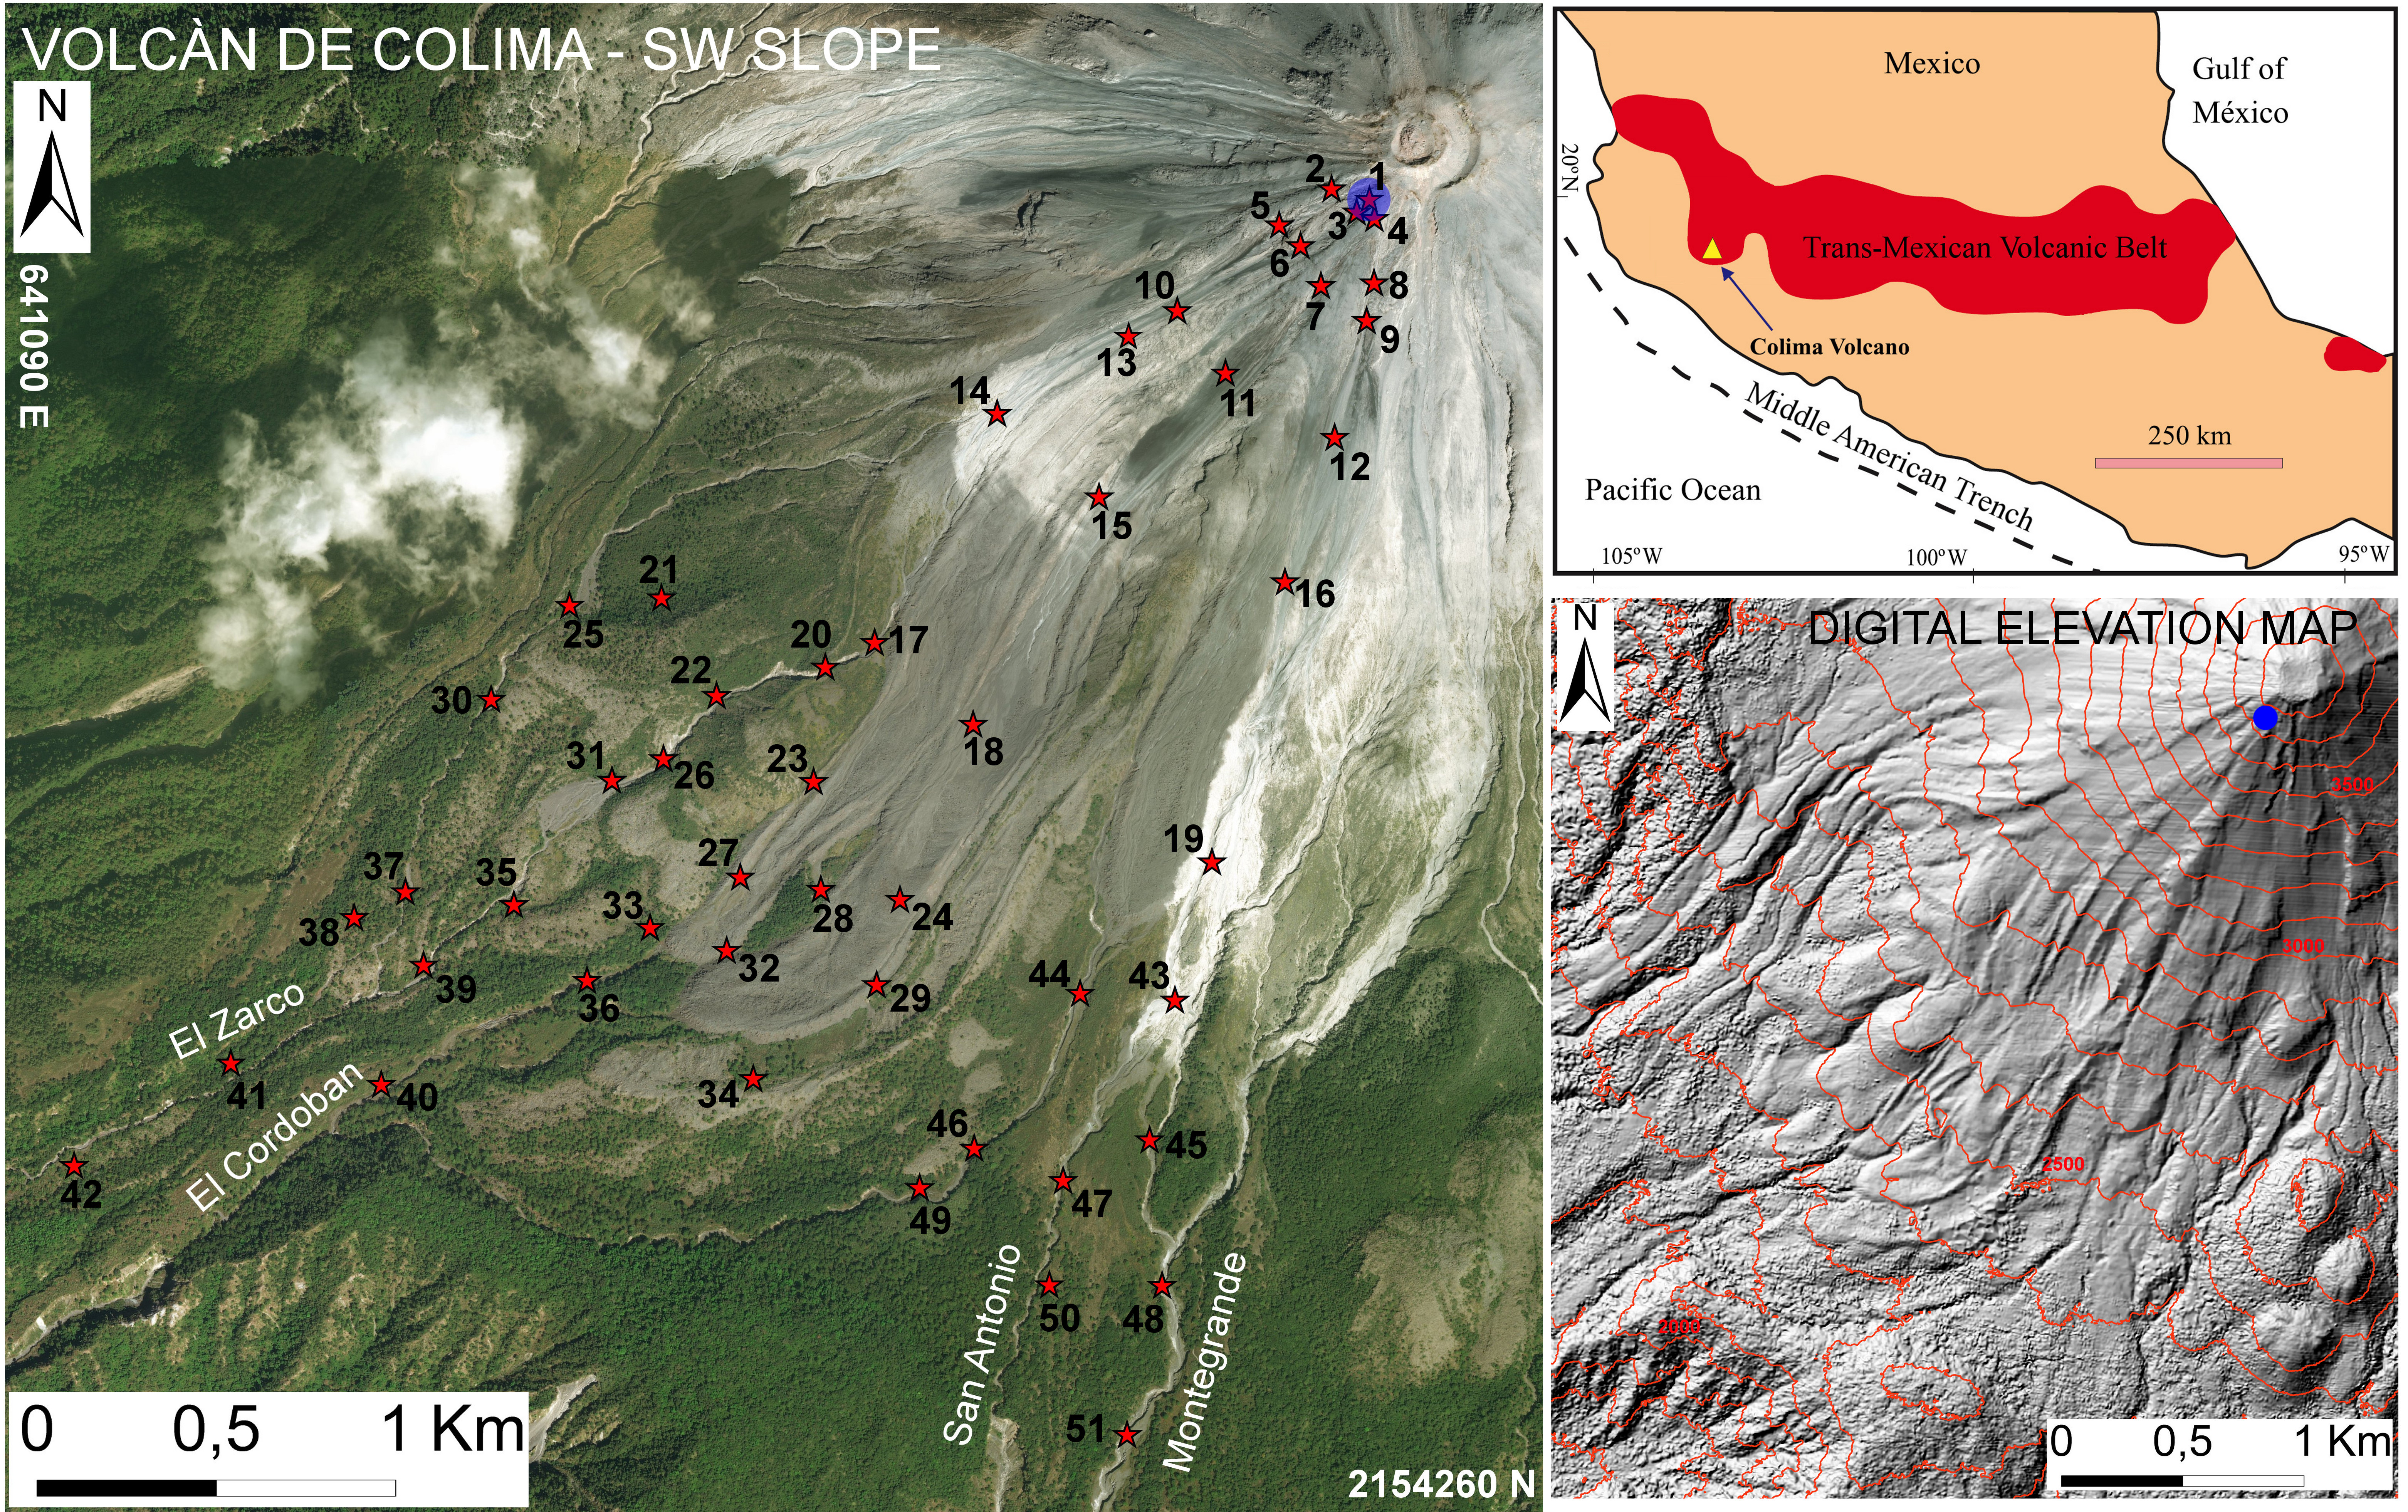
\includegraphics[width=0.9\textwidth]{BAF_VolcanDeColima/ColimaFig.jpg}
    \centering
    \caption{(a) Volc{\'a}n de Colima (M{\'e}xico) overview, including 51 numbered local sample sites (stars) and four labeled major ravines channeling the flow. Pile location is marked by a blue dot. Reported coordinates are in UTM zone 13N. Background is a satellite photo. (b) Regional geology map. (c) Digital elevation map. Six points that are adopted as preferred locations are highlighted in yellow. Elevation isolines are included in blue, elevation values in red.}
    \label{fig:Colima-first}
\end{figure}

We assume the flow to be generated by the gravitational collapse of a material pile placed close to the summit area. The volcano already produced either pyroclastic flows generated by lava dome collapse, sometimes called Merapi style flows, or by an eruptive column partial collapse, Soufriere style \citep{Macorps2017}. A dome collapse occurs when there is a significant amount of recently-extruded highly-viscous lava piled up in an unstable configuration around a vent. Further extrusion and/or externals forces can cause the still hot dome of viscous lava to collapse, disintegrate, and avalanche downhill \citep{Bursik2005, Wolpert2016}. Eruptive column collapse can occur during explosive eruptions, when the eruption column can no longer
sustain the weight of material due to loss of pressure, and hence it partially collapses down. The hot, dense blocks in this ``block and ash'' flow (BAF) will typically range from centimeters to a few meters in size. The matrix is composed of fine ash from the comminuted blocks. Computations were performed on a DEM with 5m-pixel resolution, obtained from LiDAR data acquired in 2005 \citep{Davila2007, Sulpizio2010}. We select 51 locations along the flow inundated area to accomplish local testing. Six of them are then adopted as preferred locations, being representative of different flow regimes (see Section \ref{QoI2}).


\section{Uncertainty quantification process}
\subsection{General formulation}
The key to a good forecasting capability in the context of mass flows requires the careful selection of the pair $\left(M(A), P_{M(A)}\right)$, where $A$ is a set of assumptions, $M(A)$ is the model which combines those assumptions, and $P_M$ is a probability distribution in the parameter space of $M$. For the sake of simplicity we are always taking $P_M$ uniformly distributed on selected parameter ranges.

\paragraph{Models and assumptions} An assumption is a quite general concept - for example it can be a specific equation for the internal stress, the implementation of bed curvature effects, of active-passive material stretching, or the use of a specific correction on the pressure effects. Assumptions are what makes the models being different, and each model may be seen as the combined result of a set of assumptions. Sometimes a good model contains a useless assumption that may be removed, sometimes a good assumption should be implemented inside a different model - those are usually considered as subjective choices, not data driven. Moreover, the correct assumptions may change through time, making the analysis more difficult. We provided a list of assumptions behind SWE general implementation, and behind each rheology in section \ref{sec:GeoPhFlows}.

\paragraph{Parameters ranges} It is worth mentioning that whereas the support of $P_M$ can be restricted to a single point in case an inverse problem is solved for the optimal reconstruction of a particular flow, this is not possible if we are interested in the general predictive capabilities of the model, i.e. the target of probabilistic hazard assessment. In this study we always assume $P_M\sim \bigotimes_{i=1}^{N_M} Unif(a_{i,M},b_{i,M})$, where $N_M$ is the number of parameters of $M$. These parameter ranges will not be selected under the influence of a particular observation, but we will try to use the information gathered in literature about the physical meaning of those values, together with a preliminary testing, aligning the range of possible runouts. This alignment step is detailed in section \ref{consistency}, and required to focus the statistical comparison on a consistence range of flow regimes.

\paragraph{Simulated quantities} The simulation algorithms can be schematized as:
$$\textmd{(1)INPUT VARIABLES} \rightarrow \textmd{(2)DYNAMIC QUANTITIES} \rightarrow \textmd{(3)OBSERVABLE OUTPUTS}$$
The \emph{input variables} are the parameters of $M$, i.e. volume, rheology coefficients, but can include also the initiation site and geometry, and the digital elevation map. The \emph{dynamic quantities} include the stress terms in the Newton Equations that rule the simulation, and their powers. Those are hidden to the observation in a real flow, but they directly depend on the parameters, and represent a fundamental link between the parameters and the observable outputs. Moreover, the models share some of those terms while change others, and this enables a detailed comparison of the real physics below the curtain (see Sections \ref{Hq1},\ref{Hq2}). Finally, the \emph{observable outputs} include what can be measured in space and time: e.g. flow height, lateral extent, area, velocity, acceleration, and combined quantities as $Fr$ (see Sections \ref{Obs1}, \ref{Obs2}). In the sequel (2) and (3) are also called quantities of interest (QoI).

\paragraph{Monte Carlo simulation} In general, for each QoI, during a Monte Carlo simulation we sample the input variables and obtain a family of temporal graphs on time domains depending on the flow duration. These results are statistically summarized - plotting their expectation, and their 5$^{\mathrm{th}}$ and 95$^{\mathrm{th}}$ percentiles. In the following, we will detail the considered input variables and quantities of interest for each of our cases study.

Our sampling technique of the input variables is based on the Latin Hypercube Sampling (LHS) idea, and in particular, on the improved space-filling properties of the orthogonal array-based Latin Hypercubes (see Appendix A). The LHS is performed over $[0,1]^3$ for the MC and VS input parameters, and $[0,1]^4$ for PF input parameters (see Section \ref{consistency}). Those adimensional samples are homothetically transformed to fill the required intervals.

\paragraph{Local samples and spatial averaging}
The QoI in the previous scheme which are evolving fields $f(\underline{\textbf x},t)$ in space-time, can be either \emph{locally sampled} or \emph{spatially integrated} (see sections \ref{sec:QoIs}, \ref{QoI2}). The spatial integral is defined by $F(t)=\int_{\mathbb R^k}f(\underline{\textbf x},t) d\underline{\textbf x}$. In the most of the cases $k=2$, and $d\underline{\textbf x}$ is given by the area of the mesh elements. Sometimes $k=3$, e.g. concerning speed, and $d\underline{\textbf x}$ is the element of volume corresponding to the mesh elements.

A fundamental part of this research was made possible by the new implementation of a local sampling option in the TITAN2D cyber-infrastructure. In particular, once a set of sample points $(x_i)_{i=1,...,N}$ is chosen, each field $f(\underline{\textbf x},t)$ is calculated as a function of time on the elements of the numerical mesh which are found to contain the $(x_i)_{i=1,...,N}$. Exploring differences in time and location enable to constrain the changes in flow regime. Those are really important because if the flow behavior is radically different, then the significance and effects of the assumptions may also change.

\paragraph{Statistical analysis of dynamical quantities}
Let $(F_i(x,t))_{i=1,\dots, 4}$ be an array of force components, where $x\in\mathbb R^2$ is a spatial location, and $t\in T$ is a time instant. The degree of contribution of those force terms can be significantly variable in space and time, and we define the
\emph{dominance factors} $(p_j)_{j=1,\dots, k}$, i.e. the probability of each $F_j$ to be the dominant force at $(x,t)$. Those probabilities tell what is chance of being the greater force term, and hence can provide a concise statistical description of the model dynamics. The dominance factors can be adopted to define a statistical decomposition of the contributions of the forces, as detailed in Appendix B. In sections \ref{stat1} and \ref{stat2} we report the dominance factors plots, to read the dynamic significance of the forces as a function of time and location.

\subsection{Forces terms definition}\label{sec:Fterms}
Forces analyzed have been classified according to the terms of the momentum equation in (\ref{eq:D_A}). Moreover, the forces terms in $S_x$ have been additionally classified, accordingly to equations (\ref{S_terms_MC}), (\ref{eq:S_terms_PF}), (\ref{eq:S_terms_VS}), describing the three rheology models considered in this study. What follows is a summary of the force terms, and this notation will be used in the following (see Sections \ref{Hq1}, \ref{Hq2}). In our case study, we focus on the right-hand side terms in the momentum equation. The analysis of $RHS$ will inform on local effects, while focusing instead on the $LHS$ would concern the exploration of un-local dynamics in space and time.

\paragraph{Left-hand side, LHS forces}
These terms are not detailed further in this study, but are included for the sake of completeness.
\begin{align}
\boldsymbol{LHS_1} = \left[\frac{\partial}{\partial t} (h\bar{u}), \frac{\partial}{\partial t} (h\bar{v})\right],
\end{align}
it is the temporal derivative of momentum.

\begin{align}
\boldsymbol{LHS_2} = \left[\frac{\partial}{\partial x}\left(h\bar{u}^2 + \frac{1}{2}k g_{z}h^2\right) + \frac{\partial}{\partial y}(h\bar{u}\bar{v}),\frac{\partial}{\partial x}(h\bar{u}\bar{v}) +
\frac{\partial}{\partial y}\left(h\bar{v}^2 + \frac{1}{2}k g_{z}h^2\right)\right],
\end{align}
it is the material derivative of momentum, due to the advection.

\paragraph{Right-hand side, RHS forces}
These terms are explored in detail in the next sections.
\begin{align}
\boldsymbol{RHS_1} = [g_x h,g_y h],
\end{align}
it is the gravitational force term, it has the same formulation in all models.

The formula of basal friction force $\boldsymbol{RHS_2}$ depends on the model:
\begin{align}
\boldsymbol{RHS_2} = -h g_z\tan(\phi_{bed})\left[\frac{\bar{u}}{\| \underset{^\sim}{\bar{\textbf u}} \|}, \frac{\bar{v}}{\| \underset{^\sim}{\bar{\textbf u}} \|} \right],\textmd{ in MC model.}\nonumber\\
\boldsymbol{RHS_2} = - h g_z \ \mu_{b}(\|\underset{^\sim}{\bar{\textbf{u}}} \| , h)\left[\frac{\bar{u}}{\| \underset{^\sim}{\bar{\textbf{u}}} \|}, \frac{\bar{v}}{\| \underset{^\sim}{\bar{\textbf{u}}} \|}\right],\textmd{ in PF model.}\\
\boldsymbol{RHS_2} = -h g_{z} \mu\left[\frac{\bar{u}}{\| \underset{^\sim}{\bar{\textbf u}}\|} , \frac{\bar{v}}{\| \underset{^\sim}{\bar{\textbf u}}\|}\right],\textmd{ in VS model.}\nonumber
\end{align}

The formula of the force related to the topography curvature, $\boldsymbol{RHS_3}$, also depends on the model:
\begin{align}
\boldsymbol{RHS_3} = -h \tan(\phi_{bed})\left[\frac{\bar{u}^3}{r_x\| \underset{^\sim}{\bar{\textbf{u}}} \|}, \frac{\bar{v}^3}{r_y\| \underset{^\sim}{\bar{\textbf{u}}} \|}\right],\textmd{ in MC model.}\nonumber\\
\boldsymbol{RHS_3} = -h\ \mu_{b}(\|\underset{^\sim}{\bar{\textbf{u}}} \|,h)\left[\frac{\bar{u}^3}{r_x\| \underset{^\sim}{\bar{\textbf{u}}} \|}, \frac{\bar{v}^3}{r_y\| \underset{^\sim}{\bar{\textbf{u}}} \|}\right],\textmd{ in PF model.}\\
\boldsymbol{RHS_3} = -h \mu\left[\frac{\bar{u}\| \underset{^\sim}{\bar{\textbf u}} \|}{r_{x}},\frac{\bar{v}\| \underset{^\sim}{\bar{\textbf u}} \|}{r_{y}}\right],\textmd{ in VS model.}\nonumber
\end{align}

All the three models have an additional force term, having a different formula and meaning in the three models:
\begin{align}
\boldsymbol{RHS_4} =  - h k_{ap}\sin(\phi_{int})\left[ \ {\rm sgn}(\frac{\partial \bar{u}}{\partial y}) \frac{\partial (g_z h)}{\partial y},\ {\rm sgn}({\frac{\partial \bar{v}}{\partial x}}) \frac{\partial (g_z h)}{\partial x}\right],\textmd{ in MC model.}\nonumber\\
\boldsymbol{RHS_4} = g_{z}h\left[\frac{\partial h}{\partial x}, \frac{\partial h}{\partial y}\right],\textmd{ in PF model.}\\
\boldsymbol{RHS_4} = -\frac{\| \underset{^\sim}{\textbf g} \|}{\xi}\| \underset{^\sim}{\bar{\textbf u}} \|^2\left[\frac{\bar{u}}{\| \underset{^\sim}{\bar{\textbf u}}\|} \ ,\frac{\bar{v}}{\| \underset{^\sim}{\bar{\textbf u}}\|}\right],\textmd{ in VS model.}\nonumber
\end{align}

\subsection{Alignment and consistency of the input ranges}\label{consistency}
In general, the three rheologies considered in this study, MC, PF, and VS, have totally different parameters. The statistical testing we perform requires to choose the parameter range $P_M$, and in principle it may be arbitrary. Nevertheless, if the total frictions of the models are not covering a similar span, the statistical comparison is dominated by trivial macroscopic differences, and cannot focus on the rheology details. Some degree of parameter consistency is required between the models.

We can find several instances of parameter choices in literature, and in general the choice depends on the case study. In all the models it is defined a basal friction stress (see $RHS_2$ in in \ref{sec:QoIs}). However, PF interpolates different effective friction angles, while VS includes a velocity based additional term. We tested that a direct correlation of effective friction angles is problematic to do. Hence, we did not follow such approach. In contrast, we make a preliminary testing on the extreme values of the parameter space, i.e. giving \emph{\textbf{max volume -- min resistance}}, and \emph{\textbf{min volume -- max resistance}}.

\paragraph{General definitions}
We assume what follows to simplify testing. Except when differently specified, parameters are sampled uniformly in linear scale.
\begin{itemize}
\item Material Volume $V$ is an additional input parameter in all the models, on the same range.

\item In MC, sampled input parameters are $\phi_{bed}$, and $\Delta \phi:=\phi_{int}-\phi_{bed}$. In particular, $\Delta \phi \in [2^{\mathrm{\circ}}, 10^{\mathrm{\circ}}]$ \citep{Dalbey2008}.

\item In PF, sampled input parameters are $\phi_1$, $\Delta \phi_{12}:=\phi_2-\phi_1$, and $\beta$. In particular, $\Delta \phi_{12} \in [10^{\mathrm{\circ}}, 15^{\mathrm{\circ}}]$, and $\beta \in [0.1, 0.85]$. Moreover, $\phi_3=\phi_1+1^\mathrm{\circ}$, and $\mathcal{L}$ is equal to 1 dm and 1 mm in the two case studies, respectively \citep{PouliquenForterre2002,ForterrePouliquen2003,Gray2014, Barker2015}.

\item In VS, sampled input parameters are $\mu$, and $\xi$. In detail, $\xi$ uniform sampling is accomplished in log-scale. In fact, values of $\xi$ between 250 and 4,000 $m/s^2$ have been described for snow avalanches \citep{Salm1993,Bartelt1999,Gruber2007}.
\end{itemize}
In summary, MC and VS have three-dimensional parameter spaces, while $PF$ a four-dimensional parameter space.

\newpage
\paragraph{Flow down an inclined plane}
In this case study, \cite{Dalbey2008} assumed $\phi_{bed}=[15^\mathrm{\circ}, 30^\mathrm{\circ}]$, while \cite{WebbBursik2016} performed a series of laboratory experiments and found $\phi_{bed}=[18.2^\mathrm{\circ}, 34.4^\mathrm{\circ}]$. We relied on those published parameter choices to decide a comprehensive parameter range. Figure \ref{fig:Ramp-MaxMinRunouts} displays the maps of max flow height and max velocities observed in the extreme cases tested. Simulation options are - max\_time = 2 s, height/radius = 1.34, length\_scale = 1 m, number\_of\_cells\_across\_axis = 10, order = first, geoflow\_tiny = 1e4 \citep{Patra2005,Aghakhani2016}. Initial pile geometry is cylindrical.

\begin{itemize}
\item \textbf{Material Volume:} $[449.0 \ ,\ 607.0] \ cm^3$, i.e. average of $528.0 \ cm^3$ and uncertainty of $\pm15\%$.
\item \textbf{Rheology models' parameter space:}

The parameter ranges adopted in this case study are:

\vskip.3cm\noindent \textbf{MC} - $\phi_{bed} \in [18^{\mathrm{\circ}}, 30^{\mathrm{\circ}}]$.

\vskip.3cm\noindent \textbf{PF} - $\phi_1 \in [10^{\mathrm{\circ}}, 22^{\mathrm{\circ}}]$.

\vskip.3cm\noindent \textbf{VS} - $\mu \in [0.22, 0.45]$, $\quad \log(\xi) \in [3, 4]$.
\end{itemize}

Even if maximum and mininum runout are both matching, the shape and lateral extent of the flow is remarkably different in the max. runout case, according to the three models. In particular, MC model can produce the largest lateral extent, and VS model displays an accentuated wedge-like shape, due to the increased friction in the lateral margins. These features will be detailed in Section \ref{Obs1}.

\begin{figure}[H]
	\centering
    \includegraphics[width=0.9\textwidth]{Figures/MaxMinRunout.png}
    \caption{Inclined plane setup. Contours of $h = 1.0$ mm at last simulated snapshot ($t = 1.5$ sec) for simulated flows with \emph{minimum runout} obtained from \emph{\textbf{min volume -- max resistance}}, and \emph{maximum runout} obtained from \emph{\textbf{max volume -- min resistance}}. {\color{red} \textbf{---}} : MC, {\color{blue} \textbf{---}} : PF, \textbf{---} : VS.}\label{fig:Ramp-MaxMinRunouts}
\end{figure}

\newpage
\paragraph{Volc{\'a}n de Colima block and ash flow}
In this case study, \cite{Dalbey2008} assumed $\phi_{bed}=[15^\mathrm{\circ}, 35^\mathrm{\circ}]$, while \citep{Capra2011} adopted $\phi_{bed}=30^\mathrm{\circ}$ in the simulation of a BAF in that same setting. Moreover, \cite{Spiller2014,Bayarri2015,Ogburn2016} found a statistical correlation between flow size and effective basal friction inferred from field observation of geophysical flows. The size of the BAF of this study would have $\phi_{bed}=[13^\mathrm{\circ}, 18^\mathrm{\circ}]$ according to their estimates. Figure \ref{Colima-MaxMinExtents} displays the maps of max flow height and max velocities observed in the extreme cases tested. Simulation options are - max\_time = 7200 s (2 hours), height/radius = 0.55, length\_scale = 4e3 m, number\_of\_cells\_across\_axis = 50, order = first, geoflow\_tiny = 1e4 \citep{Patra2005,Aghakhani2016}. Initial pile geometry is paraboloid.

\begin{itemize}
\item \textbf{Material Volume:} $[2.08, 3.12] \times 10^5 \ m^3$, i.e. average of $2.6  \times 10^5 \ m^3$ and uncertainty of $\pm 20\%$.
\item \textbf{Rheology models' parameter space:}

The parameter ranges adopted in this case study are:

\vskip.3cm\noindent \textbf{MC} - $\phi_{bed} \in [10^{\mathrm{\circ}}, 25^{\mathrm{\circ}}]$.

\vskip.3cm\noindent \textbf{PF} - $\phi_1 \in [8^{\mathrm{\circ}}, 18^{\mathrm{\circ}}]$.

\vskip.3cm\noindent \textbf{VS} - $\mu \in [0.15, 0.45]$, $\quad \log(\xi) \in [1.7, 4]$.

\end{itemize}

The models possess different features, even if the maximum runuout after channelization in the ravines is matching. In particular, VS lateral spreading is significant lower and material reaches higher thickness, whereas PF model seems to stop more gradually than MC with a more complex inundated area boundary lines. These features will be detailed in Section \ref{Obs2}.

\begin{figure}[H]
         \centering
        \includegraphics[width=0.87\textwidth]{Figures/ExtremeMaps.jpg}
        \caption{Volc\'an de Colima BAF. Comparison between \emph{max flow height} maps of simulated flow, assuming Mohr-Coulomb (a),(b), Pouliquen-Forterre (c),(d), and Voellmy-Salm (e),(f) rheology. Extreme cases producing maximum and minimum runout, i.e. (a),(c),(e) \emph{\textbf{max volume -- min resistance}} and (b),(d),(f) \emph{\textbf{min volume -- max resistance}}.}
        \label{Colima-MaxMinExtents}
\end{figure}

\section{Results of small scale flows on inclined plane and flat runway}\label{sec:QoIs}
First case study is the small scale experimental setting described above. First we describe the observable outputs (Section \ref{Obs1}), and then the hidden dynamic quantities (Section \ref{Hq1}). In many plots we note the effect of cutting the flow when height is $<1$ mm, which is at the scale of the smallest granular size. Continuity assumption would not be valid below this scale. In particular, in Fig. \ref{fig:Ramp-H} both the 5$^{\mathrm{th}}$ and 95$^{\mathrm{th}}$ percentile plots are vertically cut to zero when they decrease over that threshold. The mean plot is not cut to zero but it is dulled by this cutoff.

\subsection{Observable outputs} \label{Obs1}
Observable outputs include the flow height, speed, $Fr$, and acceleration as a function of time, measured on the four location $L_1,\dots, L_4$ displayed in Fig. \ref{fig:Ramp-first}. In addition, max lateral extension, flow area, and spatially averaged speed and $Fr$ are displayed. Uncertainty quantification (UQ) is also performed, accordingly to the parameter ranges described in Section \ref{consistency}.

\newpage
\subsubsection{Flow height}
Figure \ref{fig:Ramp-H} shows the flow height, $h(L,t)$, at the points $(L_i)_{i=1,\dots,4}$, for the three rheology models.
\begin{figure}[H]
         \centering
        \includegraphics[width=1\textwidth]{InclinedPlane/LocalMeasurments/Height.png}
        \caption{Records of flow height at four spatial locations of interest. Bold line is mean value, dashed/dotted lines are 5$^{\mathrm{th}}$ and 95$^{\mathrm{th}}$ percentile bounds. Different rheology models are displayed with different colors. Plots are at different scale, for simplifying lecture.}
        \label{fig:Ramp-H}
\end{figure}
In plot \ref{fig:Ramp-H}a, related to point $L_1$ placed on the initial pile, the initial values of $\sim 6\pm 1$ cm are the equal and only represent the assigned pile height. Then the flow height decreases slightly faster for the PF model, and slower for the MC, compared to the VS. Differences are more significant in plot \ref{fig:Ramp-H}b, related to point $L_2$, placed in the middle of the slope. Maximum flow height is greater for the VS, $4.1\pm 0.2$ mm, more uncertain for the MC $3.9\pm 0.4$ mm, and smaller for the PF model $3.0\pm 0.1$ mm. After the peak, PF decreases significantly slower than the other models. These height values are about 15 times smaller than initial pile height. None of the models leaves a material deposit in $L_1$ or $L_2$, and hence the 95$^{\mathrm{th}}$ percentile of the height is null at the ending-time. In contrast, a deposit is left at points $L_3$ and $L_4$, i.e. plot \ref{fig:Ramp-H}c placed at the change in slope, and plot \ref{fig:Ramp-H}d in the middle of the flat runout. At $L_3$ MC's deposit, $2$ mm with uncertainty [-2,+8] mm, is higher than the other models'. The plot profile is bimodal, showing a first peak at $\sim 0.6$ s, and then a reduction until $1$ s, before the final accumulation. At $L_4$,deposit it is not significantly different between the three models. It is of $\sim 3$ mm in average, slightly larger in VS, with uncertainty [-3,+7] mm. In general, it is observed the elimination of material when flow height is $<1$ mm.

\subsubsection{Flow speed}
Figure \ref{fig:Ramp-Vel} shows the flow speed, $\Vert \underline{\mathbf{u}} \Vert(L,t)$, at the points $(L_i)_{i=1,\dots,4}$, for the three rheology models.
\begin{figure}[H]
         \centering
        \includegraphics[width=1\textwidth]{InclinedPlane/LocalMeasurments/Velocity_Inc.png}
        \caption{Records of flow speed at four spatial locations of interest. Bold line is mean value, dashed/dotted lines are 5$^{\mathrm{th}}$ and 95$^{\mathrm{th}}$ percentile bounds. Different rheology models are displayed with different colors. Plots are at different scale.}
        \label{fig:Ramp-Vel}
\end{figure}
In plot \ref{fig:Ramp-Vel}a related to point $L_1$ speed peaks are $0.95 \pm 0.3$ m/s in MC, $1.1 \pm 0.2$ m/s in VS and PF. VS speed decreases almost linearly, while MC and PF have a more concave profile, making MC the faster model after $0.3$ sec. Plot \ref{fig:Ramp-Vel}b, related to point $L_2$, the peaks are $0.65 \pm 0.2$ m/s in MC, $0.7 \pm 0.1$ m/s in VS, and $0.52 \pm 0.08$ m/s in PF. In this case it is the PF model to decrease more linearly. In plot \ref{fig:Ramp-Vel}c, related to point $L_3$, peak velocity is $0.48$, $[+0.24, -0.20]$ m/s in MC, $0.54$, $[+0.1, -0.06]$ m/s in VS, and $0.36$, $[+0.06, -0.04]$ m/s in PF. In plot \ref{fig:Ramp-Vel}d, related to point $L_4$, peak velocity is $0.48$, $[+0.34, -0.48]$ m/s in MC, $0.48\pm 0.24$ m/s in VS, and $0.26$, $[+0.12, -0.26]$ m/s in PF. In all cases UQ shows that MC model uncertainty is remarkably larger than in the other models, and produces higher values in the 95$^{\mathrm{th}}$ percentile plots. Lowest speed values are affected by the elimination of material below $1$ mm flow height threshold. After $0.05$ s, the PF velocity profile is always significantly lower than the other models, but it also decreases slower, and matches with the stopping times of them. Moreover, it is worth noting that, curiously, PF reaches the points earlier. Speed in the deposits is below $0.1$ m/s in $L_3$, negligible in $L_4$.

\subsubsection{Froude Number}
Figure \ref{fig:Ramp-Fr} shows the Froude Number, $\Vert \underline{\mathbf{u}} \Vert/\sqrt{gh}$, at the points $(L_i)_{i=1,\dots,4}$, for the three rheology models.
\begin{figure}[H]
         \centering
        \includegraphics[width=1\textwidth]{InclinedPlane/LocalMeasurments/Froude.png}
        \caption{Records of Froude number at four spatial locations of interest. Bold line is mean value, dashed/dotted lines are 5$^{\mathrm{th}}$ and 95$^{\mathrm{th}}$ percentile bounds. Different rheology models are displayed with different colors. Plots are at different scale.}
        \label{fig:Ramp-Fr}
\end{figure}
Froude Number combines the estimates of flow height and speed, described above. In plot \ref{fig:Ramp-Fr}a, related to point $L_1$, $Fr$ maximum average value is smaller for the MC model, $\sim 4$, than for the others, $\sim 6$. However, UQ tells us that 95$^{\mathrm{th}}$ percentile almost reaches $\sim 10$ in all the three models. After the peak, the values decrease slower and more concavely in MC model than in the others. In plot \ref{fig:Ramp-Fr}b, related to point $L_2$, $Fr$ shows a bimodal profile in time, with two separate peaks at $\sim 10$ on average, but reaching $\sim 18$ in the 95$^{\mathrm{th}}$ percentile plot. In fact, first maximum, at $\sim 0.25$ s is due to the speed peak, and second, at $\sim 0.6$ s is related to $\sqrt{h}$ decreasing while the speed is not significantly changing. In plot \ref{fig:Ramp-Fr}c and \ref{fig:Ramp-Fr}d, related to points $L_3$ and $L_4$, bimodality is less accentuated and becomes a plateau profile in $\sim [0.5, 0.75]$ s. PF model gives significantly larger $Fr$ values, even $>20$ at $L_3$, due to a larger speed and a thinner flow. It is worth noting, for the sake of PF model, that $Fr>\beta$ and the flow is in the dynamic regime during the most of the time.

\subsubsection{Flow acceleration}
Figure \ref{fig:Ramp-AccL} shows the flow speed, $\Vert \underline{\mathbf{a}} \Vert(L,t)$, at the points $(L_i)_{i=1,\dots,4}$, for the three rheology models.
\begin{figure}[H]
         \centering
        \includegraphics[width=1\textwidth]{InclinedPlane/LocalMeasurments/Acceleration.png}
        \caption{Records of flow acceleration magnitude (computed from LHS). Bold line is mean value, dashed lines are 5$^{\mathrm{th}}$ and 95$^{\mathrm{th}}$ percentile bounds. Different rheology models are displayed with different colors. Plots are at different scale.}
        \label{fig:Ramp-AccL}
\end{figure}
Acceleration is the link between force terms and observable motion. We calculated it from the LHS of the dynamical equation, but using the RHS terms produces very similar results, although not identical due to the numerical approximations in our solution. In plot \ref{fig:Ramp-AccL}a, related to point $L_1$, MC and VS show a plateau before $\sim 0.4$ sec, at $\sim 2.5 \ m/s^2$ and $\sim 3.5 \ m/s^2$, respectively, while PF linearly decreases between those same values. In plot \ref{fig:Ramp-AccL}b, related to point $L_2$, are MC and PF to show a plateau, at $\sim 2.2$ m/s$^2$, while VS has a more bell-shaped profile. UQ tells us that PF has a smaller uncertainty than the other models. In plot \ref{fig:Ramp-AccL}c, related to point $L_3$, all the models show a bimodal profile, with peaks at $\sim$ 0.5 sec and 0.8 sec. This is more accentuated for MC and VS, whereas the second peak is almost absent from PF profile. The second peak is motivated by an increase of velocity in the down-slope direction after its reduction due to lateral spreading of material. At the first peak, acceleration values are significant, with average peaks of MC and PF both at $\sim 15 \ m/s^2$, and 95$^{\mathrm{th}}$ percentile plot reaching $\sim 50 \ m/s^2$ and $\sim 55 \ m/s^2$, respectively. VS shows about halved acceleration peak values. At the second peak, average acceleration values are similar for MC and VS, at $\sim 5 \ m/s^2$. In contrast, 95$^{\mathrm{th}}$ percentile plot is $> 50 \ m/s^2$ for MC, while $\sim 30 \ m/s^2$ for VS. In plot \ref{fig:Ramp-AccL}d, related to point $L_4$, the acceleration has a first peak at $\sim 4 \ m/s^2$, and a final asymptote at $\sim 2 \ m/s^2$ for MC and VS, $\sim 1 \ m/s^2$ for PF. These values generally mean flow deceleration, and uncertainty is more relevant for MC and PF than for VS.
\begin{figure}[H]
        \centering
        \includegraphics[width=1\textwidth]{InclinedPlane/AveragedMeasurments/Averaged_MeasuresIncline.png}
        \caption{Comparison between spatial averages of $(a)$ flow speed, and $(b)$ Froude Number in addition to the flow $(c)$ lateral extent, and $(d)$ inundated area, as a function of time.}
        \label{fig:Ramp-spatial}
\end{figure}

\subsubsection{Flow extents and spatial integrals}
Figure \ref{fig:Ramp-spatial} shows the spatial average of speed and Froude Number, for the three rheology models. Moreover, it shows the (maximum) lateral extent and inundated area of flow, as a function of time. Spatial averages and global quantities as maximum lateral extent and inundated area have smoother plots than local measurements. Most of the details observed in local measurements are not easy to discern. In plot \ref{fig:Ramp-spatial}a the speed shows a bell-shaped profile in all the models, with an average peak at $\sim 1.4 m/s$ and uncertainty range, given by 5$^{\mathrm{th}}$ and 95$^{\mathrm{th}}$ percentiles, of $\pm 0.4 m/s$ for PF and VS. VS is slightly slower, reaching $\sim 1.3 m/s$ in the average. MC shows a larger uncertainty range, of $\pm 0.6 m/s$. The maximum speed is reached first by VS and PF at $\sim 0.55 s$, and last by MC at $\sim 0.65 s$. In plot \ref{fig:Ramp-spatial}b, also Froude Numbers have a bell-shaped profile. Fr peaks are temporally aligned with speed peaks, and are $\sim 10$ in VS, $\sim 11$ in MC, $\sim 13.5$ in PF, on average. Uncertainty range is about $\pm 4$ in all models. In plot \ref{fig:Ramp-spatial}c inundated area shows similar max values in PF and VS, at $\sim 0.6 m^2$ on average, and uncertainty of $\pm 0.15 m^2$. MC is lower, at $\sim 0.45 m^2$ on average, and less uncertain, $\pm 0.10 m^2$. VS does not decrease significantly after reaching the peak, whereas the other models contract their area, to approximately half of the maximum extent. In plot \ref{fig:Ramp-spatial}d the lateral extent starts equal to the pile diameter $15 cm$, and then rises in two stages in MC and PF, the second and greater rise starting at $\sim 0.6 s$, corresponding to the time of arrival at the change in slope $L_3$ (see Fig. \ref{fig:Ramp-H}c). VS rises without showing two phases. After the first phase, average lateral extent is at $\sim 50 cm$ in PF and VS, while it is $\sim 43 cm$ in MC. Uncertainty range is $\pm 7 cm$ for all models at that time. Final extent is $\sim 75 cm$ in PF, $\sim 65 cm$ in MC, $\sim 55 cm$ in VS. Uncertainty range is $\pm 5 cm$ in VS, but rises to $\pm 10 cm$ in MC and PF.

\subsection{Statistical analysis of dynamic quantities}\label{Hq1}
We focus on the force terms and related powers, as well as their statistical analysis. The classification follows the definitions in section \ref{sec:Fterms}. In particular, all the estimates assume a material density of the flow $\rho = 805 kg/m^3$. This a fixed scaling factor, and the plots aspect is not affected by its value.

\subsubsection{Forces terms}
Figure \ref{fig:Ramp-Fx-spatial} shows the spatial integral of the force terms in the slope direction, for the three rheology models. The spatial integration is performed on half spatial domain, due to the symmetry with respect to the flow central axis. In plot \ref{fig:Ramp-Fx-spatial}a $\boldsymbol{RHS_1}$ represents the effect of the gravity in all the models. It starts with a plateau at $\sim 1.3 N$ before $\sim 0.55 s$, then decreases to zero after the material crosses the change in slope. The force values are consistent with the expression $\rho \left(V/2\right) g_x$, representing half the weight of material, projected along the slope direction. Uncertainty range of $\pm 0.2 N$ on the peak values. MC decreases slower, and has a more significant uncertainty, after the change in slope. PF decreases faster. In plot \ref{fig:Ramp-Fx-spatial}b $\boldsymbol{RHS_2}$ represent the friction at the base of the flow. It is negative and opposed to the gravity. A similar profile is shared by the three models, with a first short-lasting weakening before $\sim 0.1 s$, a plateau with a small strengthening after $\sim 0.5 s$, and a final waning after $\sim 1 s$, at the conclusion of the dynamics. MC does not reach zero, while the other models do. VS values are generally $\sim 0.5 N$ weaker than MC, and PF is intermediate, except in the initial peak, where it is the weakest. Strongest forces are reached during the plateau, and are $\sim -0.55 N$, $\sim -0.75 N$, $\sim -0.9 N$, with uncertainty range of $\pm 0.25 N$ in the plateau. Uncertainty is reduced in the final stages of VS and PF, but increases in MC. In plot \ref{fig:Ramp-Fx-spatial}c $\boldsymbol{RHS_3}$ is related to the curvature effects, and is not null only at the change in slope. It is always negative, i.e. reducing flow velocity, indeed it is equivalent to the friction due to the additional weigh generated by centrifugal forces. Its scale is ten times smaller than the previous plots, with values above $0.1 N$ only in MC. VS displays a bimodal profile, with a second and weaker peak at $\sim 0.75 s$. In plot \ref{fig:Ramp-Fx-spatial}d $\boldsymbol{RHS_4}$ is related to the additional forces of the models, differently characterized. In MC and PF, they are significantly small forces before $0.1 s$, completely negligible later. In VS, this is the velocity dependent term. It is negative and plays a significant role. It reaches $\sim 1 N$ at the change in slope, with uncertainty $\pm 0.3 N$. It is bell shaped and null before $\sim 0.1 s$ and after $\sim 1 s$. In plot \ref{fig:Ramp-Fx-spatial}e $\sum^4_{i=1}\boldsymbol{RHS_i}$ represents the total force in the slope direction, and summarizes the previous plots. The profile is characterized by a positively valued stage at $\sim 0.5 N$ before the change in slope, and by a negatively valued stage after that, with bell-shaped profile, and a peak at $\sim -0.5 N$. In the first stage MC is more flat, while PF and VS decrease. In the second stage MC is occurring later in time, of $\sim 0.1 s$; PF and VS are remarkably similar, but VS wanes faster.
\begin{figure}[H]
        \centering
        \includegraphics[width=1\textwidth]{InclinedPlane/AveragedMeasurments/ForcesIncline.png}
        \caption{Spatial sum of the RHS forces in the slope direction. Bold line is mean value, dashed lines are 5$^{\mathrm{th}}$ and 95$^{\mathrm{th}}$ percentile bounds. Scale of plot (c) is ten times larger than in (a),(b),(d); scale of plot (e) is slightly smaller.}
        \label{fig:Ramp-Fx-spatial}
\end{figure}

\subsubsection{Power terms}
Figure \ref{fig:Ramp-Power-spatial} shows the spatial integral of powers, for the three rheology models. The spatial integration is performed on half spatial domain, due to the symmetry with respect to the flow central axis. The plots follow the same order used in Fig. \ref{fig:Ramp-Fx-spatial}, but the scalar product with velocity imposes the bell-shaped profile observed in Fig. \ref{fig:Ramp-spatial}a. In plot \ref{fig:Ramp-Power-spatial}a the power of $\boldsymbol{RHS_1}$ starts from zero and rises up to $\sim 1.5 W$, with uncertainty of $\pm 0.5 W$. In plot \ref{fig:Ramp-Power-spatial}b the power of  $\boldsymbol{RHS_2}$ is negative and peaks to $\sim 1 W$ in MC and PF, $\sim 0.7 W$ in VS. The initial ripple observed in Fig. \ref{fig:Ramp-Fx-spatial}b is not observed, nor the plateau. In plot \ref{fig:Ramp-Power-spatial}c the power of $\boldsymbol{RHS_3}$ has a similar profile to the force it is weaker than $-0.1 W$ on average, although MC uncertainty reaches $\sim -0.25 W$. In plot \ref{fig:Ramp-Power-spatial}d the power of $\boldsymbol{RHS_4}$ is relevant only in VS, although also in PF has a very short lasting positive peak up to $0.3 W$ before to become null at $\sim 0.1 s$. Power in VS is  $\sim -0.7 W$, $\pm 0.3 W$. In plot \ref{fig:Ramp-Power-spatial}e the power of the total force $\sum^4_{i=1}\boldsymbol{RHS_i}$ summarizes the energy accumulation and dissipation, following a sinusoid profile. As observed in Fig. \ref{fig:Ramp-Fx-spatial}e, MC profile is delayed of $\sim 0.1 s$ compared to the others, and is affected by a larger uncertainty.
\begin{figure}[H]
        \centering
        \includegraphics[width=1\textwidth]{InclinedPlane/AveragedMeasurments/PowersIncline.png}
        \caption{Spatial sum of the RHS powers. Bold line is mean value, dashed lines are 5$^{\mathrm{th}}$ and 95$^{\mathrm{th}}$ percentile bounds. Model comparison on the mean value is also displayed.}
        \label{fig:Ramp-Power-spatial}
\end{figure}

\subsubsection{Force dominance factors}\label{stat1}
Figure \ref{fig:Ramp-Pr_x} shows the Dominance Factors $(P_i)_{i=1,\dots,4}$, for the three rheology models and focusing on the RHS terms in the slope direction. The are the probability of each force term (described in section \ref{sec:Fterms}) to be the greater one. The values are probability values, hence in $[0,1]$. The plots include also the probability of no-flow in the considered point. The different models are plotted separately: \ref{fig:Ramp-Pr_x}a,d,g,j assume MC; \ref{fig:Ramp-Pr_x}b,e,h,k assume PF; \ref{fig:Ramp-Pr_x}c,f,i,l assume VS. The plots \ref{fig:Ramp-Pr_x}a,b,c are related to point $L_1$, placed on the initial pile. Only $\boldsymbol{RHS_1}$ can be the dominant force, and no-flow probability is $(1-P_1)$. Same thing in the plots \ref{fig:Ramp-Pr_x}d,e,f are related to point $L_2$, placed in the middle of the slope. The plots \ref{fig:Ramp-Pr_x}g,h,i are related to point $L_3$, placed at the change in slope. $\boldsymbol{RHS_3}$ can be the dominant term for a short time, with a peak probability of $\sim 30\%$. The plots \ref{fig:Ramp-Pr_x}j,k,l are related to point $L_4$, placed in the middle of the flat runout. Only $\boldsymbol{RHS_2}$ can be the dominant term, except in PF where there is $\sim 10\%$ that $\boldsymbol{RHS_4}$ is the dominant term at then ending-time.
\begin{figure}[H]
         \centering
        \includegraphics[width=1\textwidth]{InclinedPlane/ForceContrib/Pr_x.png}
        \caption{Records of dominance factors of \textbf{RHS} forces, in the slope direction, in four spatial locations of interest. Different rheology models are displayed with different colors. No-flow probability is also displayed with a green dashed line.}
        \label{fig:Ramp-Pr_x}
\end{figure}

\newpage
\section{Results of large scale flows on the SW slope of Volc{\'a}n de Colima (MX)}\label{QoI2}
\subsection{Observable outputs overview - Mohr-Coulomb model}
In our second case study, the number of spatial locations is significantly higher than previously. We placed 51 points to span the entire inundated area, in search of different flow regimes, displayed in Fig. \ref{fig:Colima-first}. First we show the average flow height, speed, and $Fr$ in all the locations, then, based on that, we select six points which we find representative of interesting flow regimes. Figures \ref{fig:BAF-H-MC}, \ref{fig:BAF-V-MC}, \ref{fig:BAF-Fr-MC} assume MC model, while the results related to PF and VS models are detailed on six selected points.

\subsubsection{Flow height}
Figure \ref{fig:BAF-H-MC} shows the mean flow height, $h(L,t)$, at the 51 spatial locations of interest, according to MC.
\begin{figure}[H]
         \centering
        \includegraphics[width=1\textwidth]{MC&VS_51/Height_MC2.png}
        \caption{MC model, records of average flow height, $h(L,t)$, in 51 spatial locations of interest (Fig. \ref{fig:Colima-first}).}
        \label{fig:BAF-H-MC}
\end{figure}
Different plots have different scales on either time and space axes. In plot \ref{fig:BAF-H-MC}a, the only location is set on the center of the initial pile, and the profile is similar to what observed in point $L_1$ of the inclined plane case study, in Fig.\ref{fig:Ramp-H}a. In particular, the height decreases from the initial value to zero, in about 15 s. In plots \ref{fig:BAF-H-MC}b,c,d,e, the locations are are set at less than $\sim 1$ km radius from the initial pile (projected distance, without considering slope). Their profiles are similar to point $L_2$ in Fig.\ref{fig:Ramp-H}b. The height profile is bell-shaped, starting from zero and then waning back to zero in $\sim 20$ s. All the dynamics occurs during the first minute. Plot (b) shows transitional features, and focuses on points at the boundary of the initial pile. In plots \ref{fig:BAF-H-MC}f,g,h,i,j, points are set where the slope reduces, and the flow can channelize and leave a deposit. Projected distance from the initial pile is $\sim 2-3$ km. The profiles are sometimes similar to $L_3$ of Fig.\ref{fig:Ramp-H}c, other times to $L_4$ of Fig.\ref{fig:Ramp-H}d, in a few cases showing intermediate aspects. In general is either observed an initial short-lasting bulge followed by a slow decrease lasting minutes and asymptotically tending to a positive height, or a steady increase of material height tending to a positive height. In both cases it is sometimes observed a bimodal profile in the first 5 minutes. Finally, plots \ref{fig:BAF-H-MC}k,l focus on three points set at about the runout distance of the flow, in the most important ravines, at $\sim 4-5$ km projected distance from the initial pile. Profiles are similar to what observed in point $L_4$ of Fig.\ref{fig:Ramp-H}d.

\subsubsection{Flow speed}
Figure \ref{fig:BAF-V-MC} shows the mean flow speed, $h(L,t)$, at the 51 spatial locations of interest, according to MC.
\begin{figure}[H]
         \centering
        \includegraphics[width=1\textwidth]{MC&VS_51/Velocity_MC3.png}
        \caption{MC model, records of average flow speed, $\vert\underline{u}\vert(L,t)$, in 51 spatial locations of interest (Fig. \ref{fig:Colima-first}).}
        \label{fig:BAF-V-MC}
\end{figure}
Again the different plots have different scales on either time and space axes. The plot profiles are similar to what observed in figure \ref{fig:Ramp-Vel}, following the plot profile classification described above. Maximum speed of $\sim 200 m/s$ is observed in proximity of the initial pile, in plot \ref{fig:BAF-V-MC}b, and it is related to the initiation collapse dynamics. After 1 km runout (horizontal projection), in plot \ref{fig:BAF-V-MC}e, the max speed is ten times smaller, $\sim 20 m/s$. At about 2 km from the initiation, when entering the main ravines, speed is $\sim 10 m/s$, and becomes $\sim 5 m/s$ or less in the distal part of the ravines.  In detail, in plots  \ref{fig:BAF-V-MC}f,g,h,i,j, the speed often shows bimodal profiles, not observed in the inclined plane case study. Moreover, in plots \ref{fig:BAF-V-MC}h,i,j, positive asymptotes are sometimes observed, meaning a slowly and steadily moving material even minutes after the collapse.

\subsubsection{Froude Number}
Figure \ref{fig:BAF-Fr-MC} shows the mean Froude Number, $\Vert \underline{\mathbf{u}} \Vert/\sqrt{gh}$, at the 51 spatial locations of interest, according to MC.
\begin{figure}[H]
         \centering
        \includegraphics[width=1\textwidth]{MC&VS_51/Froude_MC2.png}
        \caption{MC model, records of average Froude Number in 51 spatial locations of interest (Fig. \ref{fig:Colima-first}).}
        \label{fig:BAF-Fr-MC}
\end{figure}
Froude Number combines height and speed measurements, and plot profiles are similar to what observed in Figure \ref{fig:Ramp-Fr}. In particular, in plots \ref{fig:BAF-Fr-MC}b,c,d, strongly bimodal profile are observed due to the interplay between flow height and flow speed. In plots \ref{fig:BAF-Fr-MC}f,g,h,i,j, sharp changes are observed, and the plots are significantly rough when the speed is significantly small.

\newpage
\subsection{Observable outputs - UQ on six selected locations}\label{Obs2}
The six selected locations are $[L_8, L_{10}, L_{17}, L_{39}, L_{43}, L_{46}]$, displayed in Figure \ref{fig:Colima-extra}). First two points, $L_8$ and $L_{10}$ are both significantly close to the initiation pile, the points $L_{17}$ and $L_{43}$ are placed where the slope is reducing and the ravine channels start, and $L_{39}$ and $L_{46}$ are placed in the channels, further down-slope. Moreover, $L_8$, $L_{43}$, and $L_{46}$ are placed at the western side of the inundated area, whereas $L_{10}$, $L_{17}$, and $L_{39}$ are placed at the eastern side.
\begin{figure}[H]
         \centering
        \includegraphics[width=1\textwidth]{BAF_VolcanDeColima/FigExtra.jpg}
        \caption{Volc{\'a}n de Colima (M{\'e}xico) overview, including six selected sample sites (stars). In (a), (b), (c), (d) are enlarged the topographic features in proximity of those locations. Pile location is marked by a blue dot. Reported coordinates are in UTM zone 13N. Elevation isolines are included, at intervals of $10 m$ in black, and $100m$ in bold blue. Elevation values in red.}
        \label{fig:Colima-extra}
\end{figure}

\subsubsection{Flow height}
Figure \ref{fig:Colima-H} shows the flow height, $h(L,t)$, at the points $(L_i)_{i=8,10,17,39,43,46}$, for the three rheology models. In plots \ref{fig:Colima-H}a,b, we show the flow height in points $L_8$ and $L_{10}$, $\sim 200 m$ and $\sim 500 m$ from the initial pile, respectively. $L_8$ is on the east side, and $L_{10}$ on the west side of the flow. Models MC and PF have similar profiles, lasting less $\sim 15 s$ and bell-shaped. VS requires a significantly longer time to decrease, particularly in point $L_{10}$, where the average flow height is still positive after $\sim 200 s$. Peak average values in $L_8$ are $3.4 m$ for $PF$, $4.3 m$ for MC, $4.7 m$ for VS, with uncertainty of $\sim \pm 2 m$, halved on the lower side for $MC$, and $PF$. In $L_{10}$, models MC and PF are almost indistinguishable, with peak height at $1.4 m$ and uncertainty $\pm 0.5 m$. Model VS, in contrast, has a maximum height of $1.1 m$ lasting for $50s$, and 95$^{th}$ percentile reaching $3.7 m$. In plots \ref{fig:Colima-H}c,e, we show the flow height in points $L_{17}$ and $L_{43}$, both at $\sim 2 km$ from the initial pile, on the west and east side of the flow, respectively. All the three models show in both the points a fast spike in the first minute, followed by a slow decrease, still showing a positive average height after 30 m. Again, VS is significantly different from MC and PF, and has a secondary rise peaking at $\sim 450 s$, which is not observed in the other models. This produces higher values for the most of the temporal duration, but converges to similar deposit thickness after more than 1 hour. Maximum values are $1 m$ for MC, $2 m$ for PF, and $1.5 m$ for VS, in both locations. The 5$^{th}$ percentile is zero for all the three models, meaning that the parameter range does not always allow the flow to reach those locations. The 95$^{th}$ percentile is above $5m$ for the models, except in VS, point $L_{17}$. In plots \ref{fig:Colima-H}d,f, we show the flow height in points $L_{39}$ and $L_{46}$, both at more than $3 km$ from the initial pile, on the west and east side of the flow, respectively. The three models all show an increasing profile, except for MC in point $L_{39}$ which has an initial spike and a decrease before to rise again. A similar decreasing profile can be also observed in the 95$^{th}$ percentiles of all the models. It is significant that the 5$^{th}$ percentile of PF becomes positive after $\sim 5400 s$, meaning that the flows almost surely have reached that location. Deposit thickness is $\sim 0.5 m$ for all the models in point $L_{39}$, and $1.7 m$ for VS, $1.6 m$ for PF, $1.2 m$ for MC, in $L_{46}$.
\begin{figure}[H]
         \centering
        \includegraphics[width=1\textwidth]{BAF_VolcanDeColima/LocalMeasurments/Height.png}
        \caption{Records of flow height at six selected locations. Bold line is mean value, dashed/dotted lines are 5$^{\mathrm{th}}$ and 95$^{\mathrm{th}}$ percentile bounds. Different rheology models are displayed with different colors. Plots are at different scale, for simplifying lecture.}
        \label{fig:Colima-H}
\end{figure}

\subsubsection{Flow speed}
Figure \ref{fig:Colima-Vel} shows the flow speed, $\Vert \underline{\mathbf{u}} \Vert(L,t)$, at the points $(L_i)_{i=8,10,17,39,43,46}$, for the three rheology models. Like observed in Fig.\ref{fig:Colima-H}, pair of points $L_8$ and $L_{10}$, points $L_{17}$ and $L_{43}$, and points $L_{39}$ and $L_{46}$ have significantly similar plot profiles. In plot \ref{fig:Colima-Vel}a MC shows higher average speed, $\sim 80 m/s$, than PF and VS, both $\sim 70 m/s$. 95$^{th}$ percentile values can reach $150 m/s$ in MC, $140 m/s$ in VS, $130 m/s$ in PF. MC and PF are null after $20 s$, while VS decreases slower, and becomes null at $\sim 60 s$. In plot \ref{fig:Colima-Vel}b, the average peak values are $\sim 40 m/s$ in MC and PF, while only $20 m/s$ in VS. All the three models show 95$^{th}$ percentile values above $60 m/s$. VS speed decreases remarkably slower than in the other models, requiring more than $120 s$ to become null, while MC and PF speed remains positive for $\sim 25 s$. In plot \ref{fig:Colima-Vel}c, average speed is $\sim 20 m/s$ in PF, $\sim 10 m/s$ in MC, $\sim 2 m/s$ in VS. 95$^{th}$ percentile values can reach $\sim 55 m/s$ in PF, $\sim 48 m/s$ in MC, $\sim 24 m/s$ in VS. The duration of positive velocity in VS can be long hundredths of seconds. A very similar situation is pictured in plot \ref{fig:Colima-Vel}e. Instead in plot \ref{fig:Colima-Vel}d, only MC shows a max speed above $3 m/s$, the 95$^{th}$ percentile values at $\sim 15 m/s$. In the other models the average speed is always below $1 m/s$ and the 95$^{th}$ percentile values have an increasing profile followed by a slightly decreasing plateau, at $\sim 2 m/s$ in VS, $\sim 1 m/s$ in PF. VS can have a speed above $\sim 1 m/s$ at $\sim 3600 s$. In plot \ref{fig:Colima-Vel}f, only MC shows an average speed above zero, while in the other models even the 95$^{th}$ percentile values are always below $\sim 0.5 m/s$, and start to be positive only at $\sim 200 s$ in PF, and $\sim 600 s$ in VS. MC can have speed at $\sim 1 m/s$ for more than $\sim 500 s$, but the plot is very noisy.
\begin{figure}[H]
         \centering
        \includegraphics[width=1\textwidth]{BAF_VolcanDeColima/LocalMeasurments/Velocity_Col.png}
        \caption{Records of flow speed at six selected locations. Bold line is mean value, dashed/dotted lines are 5$^{\mathrm{th}}$ and 95$^{\mathrm{th}}$ percentile bounds. Different rheology models are displayed with different colors. Plots are at different scale. Numerical noise affecting percentile curves in (f) has been averaged.}
        \label{fig:Colima-Vel}
\end{figure}
\newpage
\subsubsection{Froude Number}
Figure \ref{fig:Colima-Fr1} shows the Froude Number, $\Vert \underline{\mathbf{u}} \Vert/\sqrt{gh}$, at the points $(L_i)_{i=8,10,17,39,43,46}$, for the three rheology models.
\begin{figure}[H]
         \centering
        \includegraphics[width=1\textwidth]{BAF_VolcanDeColima/LocalMeasurments/Froude12.png}
        \caption{Records of Froude number at six selected locations. Records of points $L_{39}$, $L_{43}$, and $L_{46}$ are displayed at two different scales, according to the initial dynamics, in plots (d-f), and the asymptotic dynamics, in plots (g-i). Bold line is mean value, dashed/dotted lines are 5$^{\mathrm{th}}$ and 95$^{\mathrm{th}}$ percentile bounds. Different rheology models are displayed with different colors.}
        \label{fig:Colima-Fr1}
\end{figure}
Froude Number is proportional on the ratio between the flow speed and the square root of flow height, and hence the observed plots profiles are the combine effects of Fig.\ref{fig:Colima-H}  and \ref{fig:Colima-Vel}. Largest values are observed when the speed is significantly high compared to the flow height. Similarly to what observed in Fig. \ref{fig:Ramp-Fr} and \ref{fig:BAF-Fr-MC}, in plots \ref{fig:Colima-Fr1}a,b bimodal profiles are displayed. The first peak when the flow arrives in the location, the second when it leaves the location. Due to the slower dynamics of VS, the bimodal profile is almost absent. In PF the peaks, at $\sim 15$ and $\sim 30$, respectively, are slightly more prominent than in MC. In contrast, in plot \ref{fig:Colima-Fr1}c, MC displays an average Fr of $\sim 15$ significantly larger than in PF, $\sim 5$, and VS is almost null. In plot \ref{fig:Colima-Fr1}e the profile is significantly similar, but with lower values. In plots \ref{fig:Colima-Fr1}d,f, only MC displays a significantly positive Fr, the average below $5$, but the 95$^{th}$ percentile can reach above $20$. Finally, in plots \ref{fig:Colima-Fr1}g,h,i, a zoom on the low Fr values in the distal locations is displayed on a long time window. Observations are sometimes noisy, and only \ref{fig:Colima-Fr1}g shows the 95$^{th}$ percentile above 1. The rest of the plots are significantly lower. In general, PF has a more decreasing and less noisy character than MC and VS, while the latter is the most noisy and also has a weakly increasing profile.

\subsubsection{Flow acceleration}
Figure \ref{fig:Colima-Accel1} shows the flow speed, $\Vert \underline{\mathbf{a}} \Vert(L,t)$, at the points $(L_i)_{i=8,10,17,39,43,46}$, for the three rheology models.
\begin{figure}[H]
         \centering
        \includegraphics[width=1\textwidth]{BAF_VolcanDeColima/LocalMeasurments/Acceleration12.png}
        \caption{Records of flow acceleration magnitude (computed from LHS), in six selected locations. Records of points $L_{39}$, $L_{43}$, and $L_{46}$ are displayed at two different scales, according to the initial dynamics, in plots (d-f), and the asymptotic dynamics, in plots (g-i). Bold line is mean value, dashed lines are 5$^{\mathrm{th}}$ and 95$^{\mathrm{th}}$ percentile bounds. Different rheology models are displayed with different colors. Numerical noise affecting percentile curves in the small box of (f) has been averaged.}
        \label{fig:Colima-Accel1}
\end{figure}
In plot \ref{fig:Colima-Accel1}a,b, MC and PF display a higher maximum acceleration, both at $\sim 6 m/s^2$ and $\sim 2.5 m/s^2$ in the first and second plot respectively, than VS, $\sim 3.5 m/s^2$ and $\sim 0.5 m/s^2$, respectively. The latter has a slower decrease to zero, consistent with what observed on the speed and Froude. Uncertainty in VS is more significant in plot \ref{fig:Colima-Accel1}a, than in plot \ref{fig:Colima-Accel1}. It is the opposite in MC and PF. In plot \ref{fig:Colima-Accel1}c, in MC and PF there can a significant peak in acceleration, up to $\sim 15 m/s^2$ and $\sim 10 m/s^2$, in the 95$^{th}$ percentile values, respectively. The same peak is absent in the average plots, which are significantly flat in all the models, with values at $\sim 1 m/s^2$ in MC and PF, and $\sim 0.5 m/s^2$ in VS, at $\sim 200 s$. Plot \ref{fig:Colima-Accel1}e is similar, but PF is significantly reduced and lack of the peak in the 95$^{th}$ percentile values. In plot \ref{fig:Colima-Accel1}d,f, only MC shows significant acceleration values. Like in Fig.\ref{fig:Colima-Fr1}, plots \ref{fig:Colima-Accel1}g,h,i, are a zoom on the acceleration values in the distal locations, displayed on a long time window of $7200 s$. The last two plots are more noisy and possess an increasing trend. All the three show, in all the models, values up to $\sim 1 m/s^2$. In general, PF acceleration tends to be lower than in the other models.

\subsubsection{Flow area and spatial integrals}
Figure \ref{fig:Colima-spatial} shows the spatial average of speed and Froude Number, for the three rheology models. Moreover, it shows the inundated area of flow, as a function of time.
\begin{figure}[H]
        \centering
        \includegraphics[width=1\textwidth]{BAF_VolcanDeColima/AveragedMeasurments/Averaged_MeasuresColima.png}
        \caption{Comparison between spatial averages of $(a)$ flow speed, and $(b)$ Froude Number, in addition to the $(c)$ inundated area, as a function of time.}
        \label{fig:Colima-spatial}
\end{figure}
Like in Fig.\ref{fig:Ramp-spatial},spatial averages and inundated area have smoother plots than local measurements, and most of the details observed in local measurements are not easy to discern. In plot \ref{fig:Colima-spatial}a the speed shows a bell-shaped profile in all the models, but whereas the values where significantly similar in the inclined plane experiment, here the maximum speed is $\sim 60 m/s$ in MC, $\sim 50 m/s$ in PF, $\sim 20 m/s$ in VS, on average. Uncertainty is $\pm 18 m/s$ in MC, similar, but skewed on the larger values in VS, $\pm 10 m/s$ in PF. In plot \ref{fig:Colima-spatial}b, the Froude profile is very similar to the speed, but the difference between Vs and the other models is accentuated. Maximum values are $\sim 50$ in MC, $\sim 38$ in PF, $\sim 5$ in VS, whereas uncertainty is $\pm 10$ in MC, $\pm 7$ in PF, and skewed $[-5, +10]$ in VS. In plot \ref{fig:Colima-spatial}c, inundated area has a first peak in MC and PF, both at $\sim 1.15 km^2$, followed by a decrease to $0.55 km^2$ and $0.7 km^2$ ,respectively, and then a slower increase up to a flat plateau at $0.9 km^2$ and $1.5 km^2$, respectively. Uncertainty is $\sim \pm 0.2 km^2$ in both MC and PF until $\sim 100 s$, and then they increase at $\pm 0.3 km^2$ and $[-0.5, +0.4] km^2$, respectively. In MC the increase on uncertainty is particularly significant at $\sim 100 s$, while it is more gradual in PF. VS has a different profile. The initial peak is significant only in the 95$^{th}$ percentile values, and occurs significantly later, i.e. at $\sim 100 s$ against $\sim 50 s$ in MC and PF. It is of $\sim 1 km^2$ on the average, but up to $\sim 1.8 km^2$ in the 95$^{th}$ percentile. The decrease after the peak is very slow and the average inundated area is never below $0.85 km^2$, and eventually reaches back to $\sim 1 km^2$. Uncertainty is $[-0.3, +0.2] km^2$.

\subsection{Statistical analysis of dynamic quantities}\label{Hq2}
The current case study does not show a preferential direction, equivalent to the slope direction of the inclined plane. Hence, we will focus on the moduli, and powers, of the force terms detailed in Section \ref{Hq1}. In particular, all the estimates assume the material density of the flow $\rho = 1800 kg/m^3$. This a fixed scaling factor, and the plots aspect is not affected by its value.

\subsubsection{Force terms}
Figure \ref{fig:Colima-F-spatial} shows the spatial sum of the force terms moduli, for the three rheology models.
\begin{figure}[H]
        \centering
        \includegraphics[width=1\textwidth]{BAF_VolcanDeColima/AveragedMeasurments/ForcesColima.png}
        \caption{Spatial sum of the RHS force terms moduli. Bold line is mean value, dashed lines are 5$^{\mathrm{th}}$ and 95$^{\mathrm{th}}$ percentile bounds.}
        \label{fig:Colima-F-spatial}
\end{figure}
The figure can be compared with Fig. \ref{fig:Ramp-Fx-spatial}, which was related to forces in the slope direction in the inclined plane case study. In plot \ref{fig:Colima-F-spatial}a $\boldsymbol{RHS_1}$ represents the effect of the gravity in all the models. It is decreasing in all the models, but more gradually in VS than in the others. Initial values are $2.8e9 N$ in all the models, uncertainty $\pm 2.5e8 N$. Force values are consistent with the material weight component along the mountain slope, and their decrease is related to the slope reduction. At $\sim 10 s$ all the models show a slowing down of the decrease, which is permanent in VS, and lasting $10 s$ in MC and PF. The latter models, reach a flat profile after $\sim 60 s$, at $6e8 N$ and $7e8 N$, respectively, and uncertainty of $\pm 2e8 N$ and $1.5e8 N$. VS, which flattens more gradually, is $1.3e9 N$ at $200 s$, uncertainty $[-7e8,+8e8] N$. In plot  \ref{fig:Colima-F-spatial}b $\boldsymbol{RHS_2}$ represents the effect of the basal friction in all the models. In MC, shows a bimodal profile, with a peak at $5 s$, and a second one at $60 s$. Both of them at $9.5e8 N$ on average, with uncertainty of $[-4e8,+5e8] N$ in the first peak, and $[-5e8,+7e8] N$ in the second. The minimum between the two peaks is at $8e8 N$ and lasts from $10 s$ to $30 s$. After the second peak there is significant decrease, reaching $6e8 N$ at $90 s$, and becoming flat. Final uncertainty is $[-4e8, +6e8] N$. In PF, the plot starts from lower initial values than in the other models, but then has a unimodal peak of $1.4e9 N$ at $40 s$, on average. Uncertainty $\pm 5e8 N$. After that, the plot decreases, reaching $7.5e8 N$ at $90 s$, and becoming flat. Final uncertainty is $\pm 3.5e8 N N$, lower than in the other models. In VS, there is slow increase until the plot reaches $1.05e9 N$ at $70 s$. Then the average force is almost flat, at $1.0e9 N$, with significant uncertainty of $[-5e8,+6e8] N$. In plot \ref{fig:Colima-F-spatial}c $\boldsymbol{RHS_3}$ represents the effect of the curvature of terrain. The three models all show a bell-shaped profile, waning to zero at $90 s$. However, MC has reaches $1.1e9 N$ at $30 s$, PF $8e8 N$ at $20 s$, VS $2.5e8 N$ at $10 s$. The rise has a similar profile, but a different duration. The decrease is more gradual in VS. Uncertainty at the peak value is $\pm 4.5e8 N$ in MC, $[-2.5e8,+3.5e8] N$ in PF, $\pm 2e8 N$ in VS. In plot \ref{fig:Colima-F-spatial}d $\boldsymbol{RHS_4}$ has a different meaning in the three models. In MC it is the internal friction term, and it has a small peak in the first second, at $1e8 N$. After that it flattens to negligible values, but shows again values at $5e7 N$ after $60 s$. In PF it is the a depth averaged correction in the hydrostatic pressure, and has a almost negligible effect only in the first second, at $5e7 N$. In VS, instead, it is the velocity dependent term, and has a very relevant effect. The plot shows a bell-shaped profile, with a peak of $1.45e9 N$ at $20 s$. Uncertainty is $[-5.5e8, +6.6e8] N$, at the peak. After that, the force gradually decreases, and is $3e8 N$ at $200 s$, on average. Uncertainty $[-3e8, +7e8] N$. In plot \ref{fig:Colima-F-spatial}d, the modulus of the total force $\sum^4_{i=1}\boldsymbol{RHS_i}$ is shown, with the complex interplay between the terms. First a steep decrease due to the domination of the gravity upon the friction, then a bell-shaped increase when the friction stops the dynamics.
\newpage
\subsubsection{Power terms}
Figure \ref{fig:Colima-Power-spatial} shows the spatial sum of the powers, for the three rheology models.
\begin{figure}[H]
        \centering
        \includegraphics[width=1\textwidth]{BAF_VolcanDeColima/AveragedMeasurments/PowersColima.png}
        \caption{Spatial sum of the RHS powers. Bold line is mean value, dashed lines are 5$^{\mathrm{th}}$ and 95$^{\mathrm{th}}$ percentile bounds. Model comparison on the mean value is also displayed.}
        \label{fig:Colima-Power-spatial}
\end{figure}
The plots follow the same order used in Fig. \ref{fig:Colima-F-spatial}, but the scalar product with velocity imposes the bell-shaped profile already observed in Fig. \ref{fig:Ramp-Power-spatial}a. In plot \ref{fig:Colima-Power-spatial}a the power of $\boldsymbol{RHS_1}$ starts from zero and rises up to $\sim 1.4e11 W$ in MC, $\sim 1.2e11 W$ in PF, $\sim 6.5e10 W$ in VS. Uncertainty is $\pm 4e10 W$ in MC, $\pm 3e10 W$ in PF, $[-4e10,+5e10] W$ in VS. In plot \ref{fig:Colima-Power-spatial}b the power of  $\boldsymbol{RHS_2}$ is negative and peaks to $\sim -6.5e10 W$ in MC, $\sim -5e10 W$ in PF, $\sim -2e10 W$ in VS. Again VS power is significantly lower than in the other models. Uncertainty is $\pm 2e10 W$ in MC, $\pm 1.5e10 W$ in PF, $[-2e10,+1e10] W$ in VS. In plot \ref{fig:Colima-Power-spatial}c the power of $\boldsymbol{RHS_3}$ has a similar profile to the force, peaking to $\sim -7e10 W$ in MC, $\sim -4.5e10 W$ in PF, $\sim 5e9 W$ in VS. Uncertainty is $[-4.5e10,+3.5e10] W$ in MC, $[-2.5e10,+2e10] W$ in PF, $[-1e10,+5e9] W$ in VS. In plot \ref{fig:Colima-Power-spatial}d the power of $\boldsymbol{RHS_4}$ is relevant only in VS, although also in PF has a very short lasting positive peak up to $5e9 W$ before to become null at $\sim 10 s$. Peak negative power in VS is  $\sim -3.5e10 W$, $[-2e10,+1e10] W$. In plot \ref{fig:Colima-Power-spatial}e the power of the total force $\sum^4_{i=1}\boldsymbol{RHS_i}$ summarizes the energy accumulation and dissipation, following, like in the inclined plane case study, a sinusoid profile. As observed in Fig. \ref{fig:Ramp-Fx-spatial}e, MC profile is delayed compared to the others, and is affected by a larger uncertainty.

\subsubsection{Force dominance factors}\label{stat2}
Figure \ref{fig:Colima-Pr1} show the Dominance Factors $(P_i)_{i=1,\dots,4}$, for the three rheology models and focusing on the RHS terms moduli, at the three selected points $L_{8}$, $L_{10}$, and $L_{17}$, closer than 1 km to the initial pile (in horizontal projection).
\begin{figure}[H]
         \centering
        \includegraphics[width=1\textwidth]{BAF_VolcanDeColima/ForceContrib/Pr1_total.png}
        \caption{Records of dominance probabilities of \textbf{RHS} force moduli, at three spatial locations of interest, in the first km of runout. Bold line is mean value, dashed/dotted lines are 5$^{\mathrm{th}}$ and 95$^{\mathrm{th}}$ percentile bounds. Different rheology models are displayed with different colors. No-flow probability is also displayed.}
        \label{fig:Colima-Pr1}
\end{figure}
The plots \ref{fig:Colima-Pr1}a,b,c and \ref{fig:Colima-Pr1}d,e,f are related to point $L_8$ and $L_{10}$, respectively. They are significantly similar. $\boldsymbol{RHS_1}$ is the dominant force with a very high chance, $P_1>90\%$. In MC and PF it is observed a small chance, i.e. $P_3=5\%-30\%$ at most, of $\boldsymbol{RHS_3}$ being the dominant force for a short amount of time, i.e. $\sim 5 s$. This occurs in the middle of the time interval in which the flow is almost surely inundating the points. In VS it is observed a $P_4=5\%$ chance of $\boldsymbol{RHS_4}$ being dominant, for a few seconds, anticipating the minimum of no-flow probability. Plots \ref{fig:Colima-Pr1}g,h,i, are related to point $L_{17}$, and the plots are split in two sub-frames, following different temporal scales. In all the models, $\boldsymbol{RHS_2}$ is the most probable dominant force, and its dominance factor has a bell-shaped profile, similar to the complementary of no-flow probability. In all the models, $\boldsymbol{RHS_1}$ has a small chance of being the dominant force. In MC, this is more significant, at most $P_1=30\%$, for $\sim 20 s$ after the flow arrival, and has again about $P_1=\%2$ chance to be dominant in $[100, 7200] s$. In PF, the chance is $P_1=15\%$ at most, and has two maxima, one short lasting at about $55 s$, and the second in $[100,500] s$. Also in VS, the chance is at most $P_1=15\%$, reached at $[300, 500] s$, but its profile is unimodal in time, and becomes lower than $P_1=2\%$ after $2000 s$. In MC and PF, $\boldsymbol{RHS_3}$ has a chance of $P_3=10\%$ of being the dominant force, for a short amount of time $[30, 50] s$ and $[40, 50] s$, respectively.

Figure \ref{fig:Colima-Pr2} show the Dominance Factors $(P_i)_{i=1,\dots,4}$, for the three rheology models, at the three selected points $L_{39}$, $L_{43}$, and $L_{46}$, over 2 km far away from the initial pile.
\begin{figure}[H]
         \centering
        \includegraphics[width=1\textwidth]{BAF_VolcanDeColima/ForceContrib/Pr2_total.png}
        \caption{Records of dominance probabilities of \textbf{RHS} force moduli, at three spatial locations of interest, after 2 km of runout. Bold line is mean value, dashed/dotted lines are 5$^{\mathrm{th}}$ and 95$^{\mathrm{th}}$ percentile bounds. Different rheology models are displayed with different colors. No-flow probability is also displayed.}
        \label{fig:Colima-Pr2}
\end{figure}
The plots \ref{fig:Colima-Pr2}a,b,c and \ref{fig:Colima-Pr2}g,h,i are related to point $L_{39}$ and $L_{46}$, respectively, and they are significantly similar. Those points are both in the most distal part of the ravines, on the western and eastern side of the inundated area, respectively. They are also similar to the dominance factors at point $L_{17}$, shown in plots \ref{fig:Colima-Pr1}g,h,i, but the no-flow probability never wanes in this case, and the probability of $\boldsymbol{RHS_2}$ being the dominant force is $P_2>90\%$ till the end of the temporal window. Moreover, $\boldsymbol{RHS_1}$ does not show any initial peak in $P_2$, and generally increases slowly, reaching at most $P_2=10\%$ chance of being the dominant force in $L_{46}$, after more than $3600 s$, in all the models. Plots \ref{fig:Colima-Pr2}d,e,f, are related to point $L_{43}$, are remarkably different. In MC, either $\boldsymbol{RHS_1}$ and $\boldsymbol{RHS_2}$ can be dominant forces, both with chances of $\sim 35\%$ in the first $200 s$. Then, $\boldsymbol{RHS_2}$ increases its chance, and becomes the only dominant force after $3600 s$. The no-flow probability is neve below $30\%$. $\boldsymbol{RHS_3}$ has a chance $P_3$ up to $35\%$ for a short amount of time, i.e. $[40, 60] s$. In PF, it is $\boldsymbol{RHS_1}$ to be the dominant force, with chance above $P_1=90\%$ until $3600 s$. $\boldsymbol{RHS_2}$ rises only in the very last amount of time, reaching $P_2=40\%$ at $7200 s$, at the same level of $P_1$. The no-flow probability is very low for the most of the temporal window, rising at $20\%$ only at $7200 s$. Both $\boldsymbol{RHS_3}$ and $\boldsymbol{RHS_4}$ have a short peak of dominance factor, at about $10\%$ for a few seconds, at $[50,60] s$. Finally, in VS the no-flow probability is never below $20\%$, and the profile is similar to MC, although $\boldsymbol{RHS_1}$ is more relevant, up to $4000 s$. The other force are almost never dominant.


\section{Discussion on the comparative anatomy of geophysical flow models}
In this section we summarize the general features which differ between the models, with the purpose of depicting a thorough identikit of them, and breaking down the effects of the modeling assumptions listed in section \ref{subsec:Models}. The main focus is on the average plots, but the uncertainty percentiles are also considered, and often they exalt the differences between the models.

\subsection{Characteristic features and their motivations}
Even in the process of the preliminary alignment of the parameter ranges, the differences features in the models already affect the shape of the inundated area, both in the small flow on the inclined plane, and in the large scale geophysical flow. In Fig. \ref{fig:Ramp-MaxMinRunouts} the max runouts display a larger lateral extent in PF, and a bent shape in VS where the lateral wings remain behind the central section of the flow. In Fig. \ref{Colima-MaxMinExtents}, the three models look clearly different both in the min-runout and in the max-runout cases. Even if the maximum runout is matched, MC displays a further distal spread before channeling, PF a larger angle of lateral spread at the initiation pile, VS is less laterally extended and looks more distally stretched, significantly channelized, and with several not-inundated spots due to minor topographical coul\'{e}es.

\subsubsection{Flow height}
Flow height gives additional insight on the model features. In Fig. \ref{fig:Ramp-H}, MC seem to be more distally stretched than the other models, and starts to deposit material earlier and closer to the initial pile. PF height is generally shorter, and displays a small temporal anticipation in its arrival at the sample points. These features are probably depending by the hydrostatic correction term, which pushes forward the material at the very beginning, during the pile collapse. Also, the interpolation between the minimum $\phi_1$ and maximum $\phi_2$ friction angles, as a function of flow height and speed, plays a role in the linear cut in the flow height profile when the flow thins on the slope. VS tends to be taller than the other models, because of the reduced lateral spreading of material. In Fig. \ref{fig:Colima-H} the large scale flow height plots allow us to classify the points according to their similarity with the fours points of the small scale flow. There is a significant feature which was not observed in the small scale flow - VS is stretched distally and temporally, and material arrives later and stays longer in the sample points. This is a consequence of the speed dependent term.

\subsubsection{Flow speed and Froude Number}
Flow speed enriches our analysis of additional details. In Fig. \ref{fig:Ramp-Vel} MC has a fatter tail, due to the already observed distal spreading of material. PF profile is more concave at the beginning, due to the combined effects of the dual bed friction angle and the hydrostatic correction. In Fig. \ref{fig:Colima-Vel} VS is confirmed to be significantly slower than the other models, after the initial collapse. Moreover, it is the only model which presents slowly moving material for all the simulation, near the initiation pile. MC shows short lasting peaks of speed even in the most distal sample points, due to the lack of a strong slowing mechanism like the secondary angle in PF, and the speed dependent term in VS. Froude Number is a function of height and speed, and confirms the features already observed. In Fig. \ref{fig:Ramp-Fr} MC is more stretched and less compact, and in Fig. \ref{fig:Colima-Fr1} it is the only model which peaks to remarkable values in the most distal sample points. Froude Number is a very efficient summary for the classification of the sample points of the large scale flow on Volc\'{a}n de Colima according to the sample points in the small scale example.

\subsubsection{Flow acceleration}
Flow acceleration brings our analysis from the mechanics to the dynamics of the flow. In Fig. \ref{fig:Ramp-AccL}, at the point $L_2$ on the slope, MC has a flat plateau, while PF is linearly decreasing, and VS is bell shaped. Those differences are a consequence of the assumptions behind the models - dual angle in PF, and speed dependent term in VS. At the slope change point $L_3$, VS and MC display a bimodal profile in the acceleration. This is not a statistical effect, but it is physically observed in single simulations. The first maximum is the head of the flow hitting the ground, while the second maximum is the accumulating material in the tail. In VS the maxima are equal, because its tail is not laterally spread and hits the ground compactly. Vice versa, PF does not show such a second peak, due to the accentuated lateral spreading in the tail. In point $L_4$ on the flat runway, the average acceleration in PF is lower than in the other models at the end of the simulation time, probably because the material stops more suddenly, and the probability of no deposit is greater. In Fig. \ref{fig:Colima-Accel1} VS decreases faster, but also displays a fatter tail in the acceleration. This is similar to what already observed in the speed, and has the same motivations. MC is reaches the most distal sample points earlier and with a more significant acceleration, as we already observed commenting the Froude Number.

\subsubsection{Flow extents and spatial integral}
In Fig. \ref{fig:Ramp-spatial} the average speed and Froude Number of the different models are significantly similar, and this points to the fact that the differing features are mostly localized in space. Inundated area in PF has a greater maximum value, because of the accentuated lateral spread. In VS the inundated area almost does not decrease from its peak, because of the strictly increasing lateral spread. Vice versa, lateral spread in MC and PF has a temporary stop when the bulk of the flow hits the ground. This is a consequence of the interplay of accumulating material and the push of new material, which is stronger in the middle than in the lateral wings. In PF lateral extent is even decreasing slightly for a short time. The hydrostatic correction term may generate the pull reducing the lateral extent. In Fig. \ref{fig:Colima-spatial} average speed and Froude Number display that VS slower speed is not a local feature. Inundated area is again significantly larger in PF.

\subsubsection{Force and power terms}
Force terms provide the decomposition of the total force, already observed in the acceleration. Power terms have several features in common with the corresponding forces. Main dissimilarity is that gravitational and basal friction powers have a profile starting from zero when the flow initiates, because the flow speed starts from zero. In Fig. \ref{fig:Ramp-Fx-spatial} the differences between models are particularly relevant in term  $\boldsymbol{RHS_4}$. Speed dependent force in VS is at least one order of magnitude larger than the maximum values of the corresponding terms in MC and PF. Those are decreasing to zero after a short time from the initiation, and are negligible until the conclusive part of the dynamics. Hydrostatic correction in PF is clearly positive in the slope direction, and contributing to drive the flow ahead, at the beginning. The effects of internal friction in MC are very small, and initially positive, then negative in the slope direction. This is motivated by an initial compression of the material during the pile collapse, followed by its stretching. It is worth remarking that $\boldsymbol{RHS_2}$ and $\boldsymbol{RHS_3}$ are both smaller in VS, due to the lower basal friction angles involved. In Fig. \ref{fig:Colima-F-spatial}, the differences are accentuated, because of the topography complexity. Gravity term is larger in VS, because a portion of the flow lingers on the higher slopes for a long time. Basal friction has a higher peak in PF, due to the effect of the interpolation of the friction angle to the larger value $\phi_2$ in several portions of the flow.

\subsubsection{Force dominance factors}
The force dominance factors illustrate the predominant force term through time and the probability of no-flow. In Fig. \ref{fig:Ramp-Pr_x} the differences between the models are minor in the inclined plane case study. In general, there is only a single dominant force, and its profile is complementary with the no-flow probability. More details can be found in the force contributions analysis (Appendix B). Only in the slope change point $L_3$ the differences are remarkable. Curvature term dominance probability is bimodal in MC and VS, and in MC the second peak is smaller. The profile is similar to the spatial average of the force term. In the flat runway, at point $L_4$, in PF the hydrostatic correction can be the dominant force with a small chance. In Fig. \ref{fig:Colima-Pr1} and \ref{fig:Colima-Pr2}, the complexity in the dominance factors is greater. At the points $L_8$ and $L_{10}$, proximal to the initiation, gravitational force is dominant with a high probability until the no-flow probability become predominant. Curvature force can be dominant in MC and PF, when the no-flow change is zero, and for a short time. Gravitational force is dominant for a much larger time, because of the longer presence of the flow. The speed dependent friction can be dominant with a small probability, at the beginning of the dynamics, when flow is faster. At the points $L_{17}$, $L_{39}$, and $L_{46}$, the basal friction is dominant with high probability. $L_{17}$ is left by the flow, whereas $L_{39}$, and $L_{46}$ have a deposit at the end with a high chance. In general, in MC the no-flow probability tends to be larger than in the other models, because part of the parameter spaces stops earlier, or completely leaves the site. Again, curvature can have a small chance to be dominant in MC and PF, when the speed is high. Point $L_{43}$ is particularly interesting. It is not close to the initiation, but it is placed right after a local hill. This location shows an intermediate regime between the proximal points and the distal ones. The no-flow probability is increasing at the end, meaning that the material is leaving the site, like in $L_{17}$. Moreover, the gravity can be dominant like in the proximal points, but also the bed friction can be dominant, and in MC and VS both the two forces have similar chances to be dominant for the most of the time of the simulation. In PF, only the gravitational force is dominant with a high chance, and the no-flow probability is almost null, meaning that there is accelerating material for the most of time. This is probably because point $L_{43}$ is placed in a place right downhill of a place where a significant amount of material stops according to that model.

\section{Conclusions}
This study presents a new statistical procedure for the comparative analysis of different models for the rheology of geophysical mass flows. The method enabled us to break down the effects of the different physical assumptions in the dynamics, providing an improved understanding of what characterizes each model. We considered a Monte Carlo simulation on a range of parameter inputs, and estimated the mean and the uncertainty range of the corresponding outputs. Fitting the results on a specific flow was thus not necessary, and the procedure unfolded the physics of the models in a general framework. We also developed the concept of force dominance factor, in the study of the force terms in the different regions of space and time. This paves the way to future research aimed at designing a new generation of algorithms, which could completely bypass the search for a unique best model. They would go beyond the concept of alternative models, first decomposing them into their characterizing features, and then focusing instead on a more flexible selection of the assumptions which are locally suitable for each specific part of the simulation.

In particular, we presented:
\begin{itemize}
  \item a short review of the assumptions characterizing three commonly used rheologies of Mohr-Coulomb, Poliquenne-Forterre, Voellmy-Salm. This included a qualitative list of such assumptions, and the breaking down of the different terms in the differential equations.
  \item a preliminary procedure for selecting the portions of the parameter ranges of the models which produced consistent outputs. This was fundamental because the model comparison cannot focus on the modeling differences if the scales of the stress tensor were on different scales.
  \item an articulated statistical framework, processing the mean, and the uncertainty range of many mechanical and dynamical quantities in the flow simulation. A new function was featured in the TITAN2D solver, capable of producing local measurements of those quantities at selected sites. Spatial integrals and spatial averages were also performed, illustrating the characteristics of the entire flow under the different models. The new concept of force dominance factors enabled a simplified description of the local dynamics.
  \item the detailed results of the procedure applied to two different case studies: an inclined plane with a flat runway, and the real DEM on the SW lope of Volc\'{a}n de Colima (MX). All the differences were quantitatively commented.
  \item a final discussion, explaining all the observed features in the results on the light of the known physical assumptions of the models, and the evolving flow regime in space and time.
\end{itemize}

Our statistical analysis based on UQ depicted three very different models, due to the different assumptions underlying to them. Compared to a classical MC model, PF lacks of internal friction and this produces an accentuated lateral spread. This is increased by the hydrostatic correction, which briefly pushes the flow ahead and laterally during the initial collapse. That force can also have some minor effects in the final deposit accumulation. The interpolation of the smaller bed friction angle $\phi_1$ with the larger value $\phi_2$, suddenly stops the flow if it thins compared to its speed. This mechanism does not allow for large velocity peaks. Instead in VS, the speed dependent friction has a great effect in reducing lateral spread and producing channeling features even due to minor ridges in topography. The flow tends to be significantly slower and more stretched in the slope direction. The effects of the different formulation of the curvature term are less impacting than the effects of the lower basal friction and speed.

The procedure may be applied to other models, or modeling assumptions. Moreover, the two case studies considered had the purpose of exploring two very different scale of flows, the first on a controlled setting, the second on a real topography. Additional research concerning other case studies, and different parameter ranges, might reveal other flow regimes, and hence differences in the consequences of the modeling assumptions under new circumstances.


\section{Appendix A: Latin Hypercubes and orthogonal arrays}
The Latin Hypercube Sampling (LHS) is a well established procedure for defining pseudo-random designs of samples in $\mathbb R^d$, with good properties with respect to the uniform probability distribution on an hypercube $[0,1]^d$ \citep{McKay1979,Owen1992b,Stein1987,Ranjan2014,Mingyao2016}. In particular, compared to a random sampling, a LHS: (i) enhances the capability to fill the d-dimensional space with a finite number of points, (ii) in case $d>1$, avoids the overlapping of point locations in the one dimensional projections, (iii) reduces the dependence of the number of points necessary on the dimensionality $d$.

\begin{definition}[Latin hypercube sampling]
Let $\Xi=\{\xi_i\ :\ i=1,\dots,N\}$ be a set of points inside the d-dimensional hypercube $C=[0,1]^d$. Let $[0,1]=\bigcup_{j=1}^{N} I_j$, where $I_j=[\frac{(j-1)}{N},\frac{j}{N}]$. Let $\xi_i=\left(\xi_i^1,\dots,\xi_i^d\right)$, and for each $k\in\{1,\dots,d\}$, let $\Xi^k=\{\xi^k_i\ :\ i=1,\dots,N\}$. Let $\lambda^d$ be the uniform probability measure supported inside $C$, called Lebesgue measure. Then $\Xi$ is a latin hypercube w.r.t. $\lambda^d$ $\Longleftrightarrow$ $\forall j\in \{1,\dots,N\}$, $\forall k\in\{1,\dots,d\}$, $\left|I_j\cap\Xi^k\right|=1$.
\end{definition}

The procedure is simple: once the desired number of samples $N\in\mathbb N$ is selected, and $[0,1]$ is divided in $N$ equal bins, then each bin will contain one and only one projection of the samples over every coordinate. The LHS definition is trivially generalized over $C=\prod^d_i [a_i, b_i]$, i.e. the cartesian product of $d$ arbitrary intervals. That will be applied in this study, defining LHS over the parameter domain of the flow models.

There are a large number of possible designs, corresponding the number of permutations of the bins in the d-projections, i.e. $d\cdot N!$. If the permutations are randomly sampled there is a high possibility that the design will have good properties. However, this is not assured, and clusters o points or regions of void space may be observed in $C$. For this reason, we base our design on the orthogonal arrays (OA) \citep{Owen1992a,Tang1993}.

\begin{definition}[Orthogonal arrays]
Let $S=\{1,\dots,s\}$, where $s\ge 2$. Let $Q\in S^{n\times m}$ be a matrix of such integer values. Then $Q$ is called an $OA(n,m,s,r)$ $\Longleftrightarrow$ each $n\times r$ submatrix of $Q$ contains all possible $1\times r$ row vectors with the same frequency $\lambda=n/s^r$, which is called the index of the array. In particular, $r$ is called the strength, $n$ the size, $(m\ge r)$ the constrains, and $s$ the levels of the array.
\end{definition}

Orthogonal arrays are very useful for defining latin hypercubes which are also forced to fill the space (or its r-dimensional subspaces) in a more robust way, at the cost of potentially requiring a larger number of points than a traditional LHS.

\begin{proposition}
Let $Q$ be an $OA(n,m,s,r)$. Then let $U\in\mathbb R^{n\times m}$ be defined as follows:
$$\forall k\in \{1,\dots,s\},\ \forall j\in \{1,\dots,m\},\ \left\{Q[\cdot,j]\ :\ Q[i,j]=k\right\} = \Pi\left(\{(k-1)\lambda s^{r-1},\dots, k\lambda s^{r-1}\}\right),$$
where $\Pi$ is a random permutation of $\lambda s^{r-1}$ elements. Then $\Xi=\{\xi_i=U[i,\cdot]\ :\ i=1,\dots,n\}$ is a LHS w.r.t to $\lambda^m$ over $C=[0,1]^m$. Moreover, let $[0,1]^r=\bigcup_{(h_1,\dots,h_r)=1}^{s} I_{(h_i)}$, where $I_{(h_i)}=\prod^r_i[\frac{(h_i-1)}{s},\frac{h_i}{s}]$. Then $\forall D=(d_1,\dots,d_r)\subseteq \{1,\dots,m\}$, let $\Xi^D=\{(\xi^{d_1},\dots,\xi^{d_r})\ :\ i=1,\dots,n\}$. We have that
$$\forall k\in \{1,\dots,s\},\ \forall (h_i\ : i=1,\dots,r)\in\{1,\dots,d\}^r,\ \left|I_{(k_i)}\cap\Xi^D\right|=\lambda.$$
\end{proposition}

For each column of $Q$ we are replacing the $\lambda s^{r-1}$ elements with entry $k$ by a random permutation of $\left((k-1)\lambda s^{r-1} + h\right)_{h\in 1,\dots, \lambda s^{r-1}}$. After the replacement procedure is done, the newly obtained matrix $U$ is equivalent to a LHS which inherits from $Q$ the property of fully covering $s^r$ equal r-dimensional hypercubes in every r-dimensional projection. Each hypercube contains $\lambda$ points. In other words, inside each r-dimensional projection, the design associated to $U$ fills the space like a regular grid at the scale of those $s^r$ hypercubes, but it is still an LHS at a finer scale, i.e. the $\lambda s^{r-1}$ one dimensional bins. A complete proof can be found in \cite{Tang1993} and it is a straightforward verification of the required properties.

However, even in an LHS based on an $OA(n,m,s,r)$, if $r<m$ what happens in the projections with dimension $r'>r$ is not controlled, and randomizing procedures are made more difficult by the additional structure imposed by the $OA$. Moreover, the total number of points necessary to achieve a full design increases with $r$, and hence is affected by dimensionality issues.

Dealing with relatively small $d$, i.e. $d\in\{3,4\}$, we adopt a LHS $U$ created by a $OA(s^d,d,s,d)$. The strength is equal to the dimension $d$, hence the design fills the entire space like a $d$ dimensional grid, but it is a LHS as well. In this case there is one point in each hypercube, and $\lambda=1$. We take $s=8$ for the 3-dimensional designs over the parameter space of Mohr-Coulomb and Voellmy-Salm models, i.e. $512$ points; we took $s=6$ for the 4-dimensional designs over the more complex parameter space of the Pouliquen-Forterre model, i.e. 1296 points.

\section{Appendix B: Force contribution coefficients, and their conditional decomposition}
The \emph{contribution coefficients} are normalized quantities related to the force terms. They are obtained dividing the force terms described in section \ref{sec:Fterms} by a dominant function $\Phi$. This is a tool to compare the different force terms, scaling the plots by the dominant function $\Phi$ - in this case in $[-1,1]$. It also represent the degree of relevance of the assumptions behind the force terms, changing as a function of time.

In general we focus on the moduli of the forces, or their projection on the slope direction. Hence, in the following the forces are scalar and not vectorial terms. It is important to remark that all the forces depend on the input variables, and they are thus considered as random variables. The definitions are not depending on the location, but all the results will significantly depend of that choice. Next notation will assume to be in a selected location $x=L_k$, where $k\ge 1$.

\begin{definition}[Contribution coefficients]
Let $(F_i)_{i\in I}$ be random variables on $(\Omega, \mathcal F, P)$, representing the considered force components in location $x$ at time $t$. Then, for each component $i$, the contribution coefficient is defined as:
$$C_i:=\mathbb E\left[\frac{F_i}{\Phi}\right],$$
where $\Phi$ is a dominating function, i.e. $\Phi\ge |F_i|$, $\forall i\in I$.
\end{definition}
The \emph{total force}, i.e $\sum_i F_i$ excluding the inertial terms, is not a good candidate for a dominating function. Indeed, the terms often have opposite signs, and their sum can be really small. Another issue is given by the existence of a subset of times $\Theta$ characterized by the absence of flow in the selected location $x$. In $\Theta$ the dominant force is null, and cannot be the denominator of a fraction.

We have tested two alternative $\Phi$ choices: $\Phi_1$ is based on the $l^1$ norm, and defined as:
$$\Phi_1:=\left\{
    \begin{array}{ll}
      \sum_i \frac{|F_i|}{2}, & \hbox{if not null;} \\
      1, & \hbox{otherwise.}
    \end{array}
  \right.$$
In contrast $\Phi_2$ is a dominant force based on the $l^\infty$ norm:
$$\Phi_2:=\left\{
    \begin{array}{ll}
      \max_i |F_i|, & \hbox{if not null;} \\
      1, & \hbox{otherwise.}
    \end{array}
  \right.$$
In particular, for a particular location $x$, time $t$, and parameter sample $\omega$, we have $C_i=0$ if there is no flow or all the forces are null. The expectation of $C_i$ is reduced by the chance of $F_i$ being small compared to the other terms, or by the chance of having no flow in $(x,t)$. Moreover, $\mathbb E[C_i]\in[-1,1]$, $\forall i$.
\begin{proposition}
Let $\Phi_k$, $k=1,2$ be the functions described above. Then they are well defined dominating function, i.e. $\Phi_k\ge |F_j|$, $\forall j,k$.
\end{proposition}
\begin{proof}
If $k=1$, the Newton equation states $\sum_{j\in J} F_j =\sum_{i\in I} F_i,$ where $(F_j)_{j\in J}$ are inertial forces, and $(F_i)_{i\in I}$ the local forces. Then, $\forall h\in I$
$$F_h=\sum_{i\neq h,\ i\in I} F_i - \sum_{j\in J} F_j.$$
And hence
$$|F_h|\le |F_h|+\sum_{i\neq k,\ i\in I} |F_i| - \sum_{j\in J} |F_j|=2\Phi_1.$$
A similar equation is valid $\forall k\in J$. If $k=2$, or if the inertial forces are not included, the proof is trivial.
\end{proof}

Furthermore, assuming $\Phi=\Phi_2$, there is a useful result explaining the meaning of those coefficients through the conditional expectation.
\begin{proposition}
Let $(F_i)_{i\in I}$ be random variables on $(\Omega, \mathcal F, P)$, representing the considered force components in location $x$ at time $t$. For each $i$, let $C_i$ be the contribution coefficient of force $F_i$, assuming $\Phi=\Phi_2$. Then we have the following expression:
$$C_i=\sum_j p_j \mathbb E\left[\frac{F_i}{|F_j|}\ \Big{|}\ \Phi=|F_j|\right],$$
where $p_j:=P\left\{\Phi=|F_j|\right\}$.
\end{proposition}

\begin{proof}
Let $Z$ be a discrete random variable such that, for each $j\in\mathbb N$, $(Z=j) \Longleftrightarrow (\Phi=|F_j|)$. Then, by the rule of chain expectation:
$$C_i=\mathbb E\left[\frac{F_i}{\Phi}\right]=\mathbb E\left[\mathbb E\left[\frac{F_i}{\Phi}\ \Big{|}\ Z=j\right]\right]=$$
$$=\mathbb E\left[\mathbb E\left[\frac{F_i}{|F_j|}\ \Big{|}\ Z=j\right]\right]=\sum_j P\left\{Z=j\right\} \mathbb E\left[\frac{F_i}{|F_j|}\ \Big{|}\ Z=j\right].$$
Moreover, by definition, $p_j=P\left\{Z=j\right\}$. This completes the proof.
\end{proof}

The last proposition brings to a conditional decomposition of the contribution coeffients, taking advantage of the \emph{dominance factors} $(p_j)_{j=1,\dots, k}$, i.e. the probability of each $F_j$ to be the dominant force in $(x,t)$.

\begin{definition}[Conditional contributions and dominance factors]
Let $(F_i)_{i=1,\dots, k}$ be random variables on $(\Omega, \mathcal F, P)$, representing arbitrary force components in location $x$ at time $t$. Then, for each pair of components $(i,j)$, the conditional contribution $C_{i,j}$ is defined as:
$$C_{i,j}:=\mathbb E\left[\frac{F_i}{|F_j|}\ \Big{|}\ \Phi=|F_j|\right],$$
where $\Phi=\Phi_2$ is the dominant force. In particular, for each component $i$, the dominance factor is defined as:
$$p_j:=P\left\{\Phi=|F_j|\right\}.$$
\end{definition}

Example of the Contribution Coefficients in the cases studies of this paper are reported in the following. They represent an additional tool to compare the different force terms, following a less restrictive approach than the Dominance Factors.

\newpage
\paragraph{Example 1 - Flow down and inclined plane}
Figure \ref{fig:Ramp-Ci_x} shows the Contributions Coefficients $(C_i)_{i=1,\dots,4}$, for the three rheology models and focusing on the RHS terms in the slope direction. The different models are plotted separately: \ref{fig:Ramp-Ci_x}a,d,g,j assume MC; \ref{fig:Ramp-Ci_x}b,e,h,k assume PF; \ref{fig:Ramp-Ci_x}c,f,i,l assume VS.
\begin{figure}[H]
         \centering
        \includegraphics[width=1\textwidth]{InclinedPlane/ForceContrib/Ci_x.png}
        \caption{Records of contribution coefficients of \textbf{RHS} forces, in the slope direction, in four spatial locations of interest. Different rheology models are displayed with different colors. Dominant function $\Phi$ is calculated based on the $l^\infty$ norm}
        \label{fig:Ramp-Ci_x}
\end{figure}
The plots \ref{fig:Ramp-Ci_x}a,b,c are related to point $L_1$, placed on the initial pile. $C_1$ and $C_2$ play the major roles, with a minor contribution $C_4$ in VS. Contributions profiles are flat plateaus that start to wane after $0.4 s$, with the rise of the probability of no-flow at the point $L_1$ (see also Fig. \ref{fig:Ramp-Pr_x}. Uncertainty is related to the no-flow times, and to the value of $C_2$. The contribution $C_4$ can be significant, as it is shown by the 95$^{\mathrm{th}}$ percentile values, but appears after $0.25 s$. The plots \ref{fig:Ramp-Ci_x}d,e,f are related to point $L_2$, placed in the middle of the slope. Again the major contributions are $C_1$ and $C_2$, with trapezoidal profile preceded and followed by no-flow. In VS, $C_4$ becomes as a significant as $C_2$, but it is bimodal instead than trapezoidal. The plots \ref{fig:Ramp-Ci_x}g,h,i are related to point $L_3$, placed at the change in slope. The contributions $C_1$ and $C_2$ are still the largest, but their profiles are bell-shaped. In VS, $C_4$ is almost identical to $C_2$. In all the models, $C_3$ is also significant, with a peak similar to $C_2$, but has a different profiles - triangular for MC and PF, bimodal for VS. In MC the decrease occurs in two stages. The uncertainty tells us that $C_3$ can also be the dominant force, for a shorter time. Due to the presence of deposit, all the contributions are small (particularly small in PF), but not zero at the ending time. The plots \ref{fig:Ramp-Ci_x}j,k,l are related to point $L_4$, placed in the middle of the flat runout. Only $C_2$ has a major role, with a bell shaped profile faster to wax than to wane. Contribution $C_4$ has a minor role in VS and PF. Uncertainty affects this force, which can be shortly the dominant term, in PF.

\newpage
\paragraph{Example 2 - Volc{\'a}n de Colima BAF}
Figure \ref{fig:Colima-Ci_1} shows the Contributions Coefficients $(C_i)_{i=1,\dots,4}$, for the three rheology models and focusing on the RHS terms moduli. The different models are plotted separately: \ref{fig:Colima-Ci_1}a,d,g assume MC; \ref{fig:Colima-Ci_1}b,e,h assume PF; \ref{fig:Colima-Ci_1}c,f,i assume VS.
\begin{figure}[H]
         \centering
        \includegraphics[width=1\textwidth]{BAF_VolcanDeColima/ForceContrib/Ci1_total.png}
        \caption{Records of contribution coefficients of \textbf{RHS} force moduli, at three spatial locations of interest, in the first km of runout. Different rheology models are displayed with different colors. Dominant factor is calculated based on the $l^\infty$ norm}
        \label{fig:Colima-Ci_1}
\end{figure}
The coefficients in the first two locations, points $L_8$ and $L_{10}$, are shown in \ref{fig:Colima-Ci_1}a,b,c and \ref{fig:Colima-Ci_1}d,e,f, respectively. Those points are close to the initial pile, in the western and eastern sectors of the inundated area. The pairs of plots related to the same model are similar. In all the models the greater contribution is given by $C_1$, significantly larger than $C_2$ and $C_3$, which have similar scales in MC and PF, while $C_2>C_3$ in VS.. $C_4$ always gives a negligible contribution, except for in VS, where it is comparable with $C_2$. In $L_8$, following PF, $C_3$ is bimodal, whereas the plot is unimodal in MC and VS, or in $L_{10}$. In $L_8$, $C_3$ is greater than in $L_{10}$, compared to the other forces. Like in the previous figures, VS shows a slower decrease of the plots, which is due to the rising probability of no-flow (see also next section). In plots \ref{fig:Colima-Ci_1}g,h,i, are shown the coefficients in $L_{17}$, about 1 km from the initial pile (in horizontal projection). The plots are split in two sub-frames, following different temporal scales - the first $100 s$ are on the left, and the rest of the temporal domain $[100, 7200] s$ is on the right. Initial dynamics is dominated by $C_2$, except for in MC, and only for a short time, $[30, 35] s$. In MC there is an initial peak of $C_2$ which is not observed in the other models.  $C_3$ has a significant size, in MC and PF, and unimodal profile. In PF, after $C_3$ wanes, at about $60 s$, also $C_4$, representing the effect of hydrostatic pressure correction, is not negligible, for $\sim 40 s$. The second part of the temporal domain, is characterized by a slow decrease of $C_2>C_1$, due to the rise of the no-flow probability.

\newpage
\bibliographystyle{apalike}
\bibliography{mybibfile}

\end{document}
